%!TEX root = ../../super_main.tex

\section{Participant Interaction}
\label{sec:participant_interaction}
\todo[inline]{overvej om der skal stå ``he'' eller ``he/she'' eller noget helt tredje}
This section will describe how the participants are able to interact with the mobile application\todo{Skriv at vi bruger Google Material Design som udgangspunkt. Så har vi nogle ``standard'' elementer og principper at gå ud fra, så vi slipper for at opfinde den dybe tallerken}. Throughout this section we will provide mockups together with the implementation of the user interface on the device. When a participant opens the mobile application, the participant is presented with an initial screen, as seen in \figref{fig:initial_screen}. The idea with this screen is to welcome the participant to the application. Currently, it does not supply the participant with any information, but one could imagine that this view would, in future iterations, provide the participant with usable information, such as progress in the current campaign, clarification of what concepts and principals the participant must know. This screen could possibly also contain some motivational factor, provided by the customers, e.g. a ``prize'' for participation.

% Initial screen
\begin{figure}[!htbp]
    \begin{subfigure}[!t]{.48\textwidth}
        \centering
        
\includegraphics[width=.7\linewidth]{mockups/homepage}
        \caption{Mockup of the initial screen.}
        \label{fig:mockup_initial_screen}
    \end{subfigure}%
    \begin{subfigure}[!t]{.52\textwidth}
    \centering
        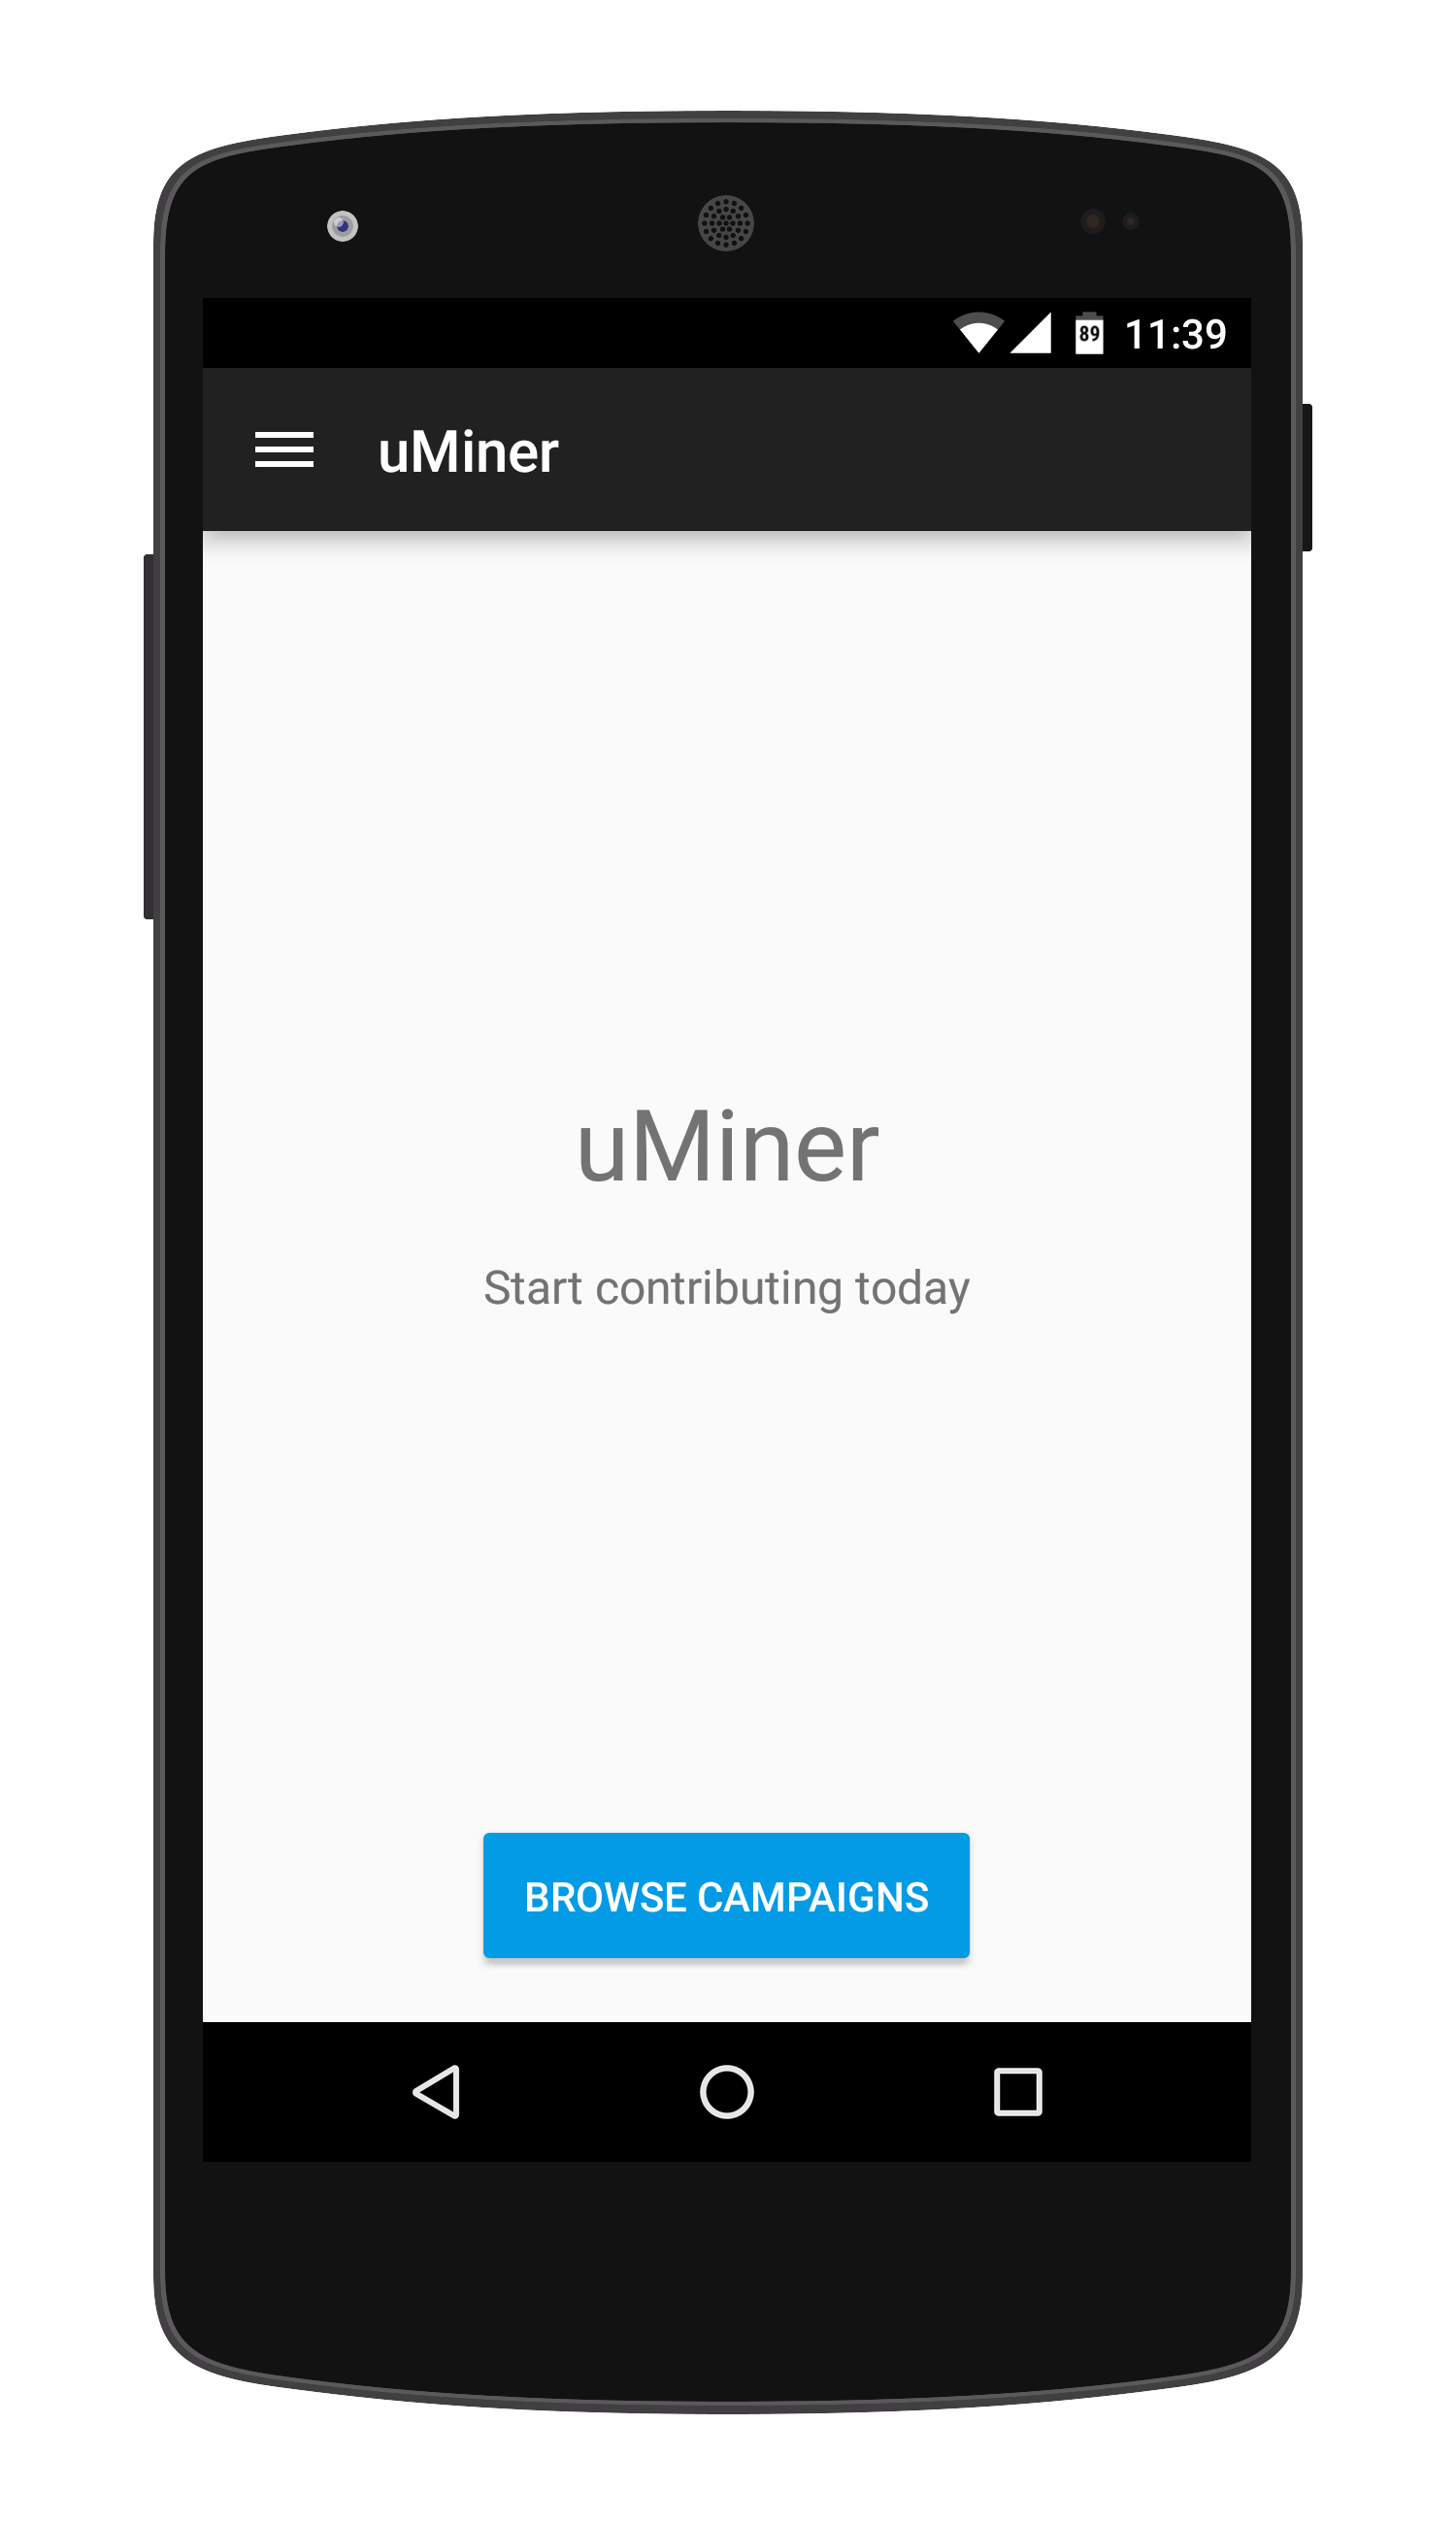
\includegraphics[width=.73\linewidth]{user_interfaces/client/client_uminer_home_with_phone}
        \caption{Implementation of the initial screen.}
        \label{fig:implementation_initial_screen}
    \end{subfigure}
    \caption{Mockup and implementation of the initial screen of the application.}
    \label{fig:initial_screen}
\end{figure}
\FloatBarrier

To navigate to other views in the application, the participants must either use the drawer menu displayed in \figref{fig:navigation} or press the \emph{browse campaigns}-button in the initial view. The navigation menu contains three elements, which will each take the participant to different parts of the application, namely ``Browse campaigns'', ``Join specific'', and ``Current campaign''.

\begin{description}
    \item[``Browse campaigns''] redirects the participant to a view containing brief information about all of the publicly available campaigns, as seen in \figref{fig:public_campaigns}.

    \item[``Join specific''] redirects the participant to a view, as seen in \figref{fig:specific_campaign}, where he/she can search for a specific campaign by providing a campaign identifier.

    \item[``Current campaign''] redirects the participant to a campaign specification view, as seen in \figref{fig:leave_campaign_no_dialog}, displaying more information about the campaign that they are currently contributing to. If the participant have not yet joined a campaign, a message will briefly be displayed on the screen, informing the participant about this.
\end{description}

% Navigation
\begin{figure}[!htbp]
    \centering
    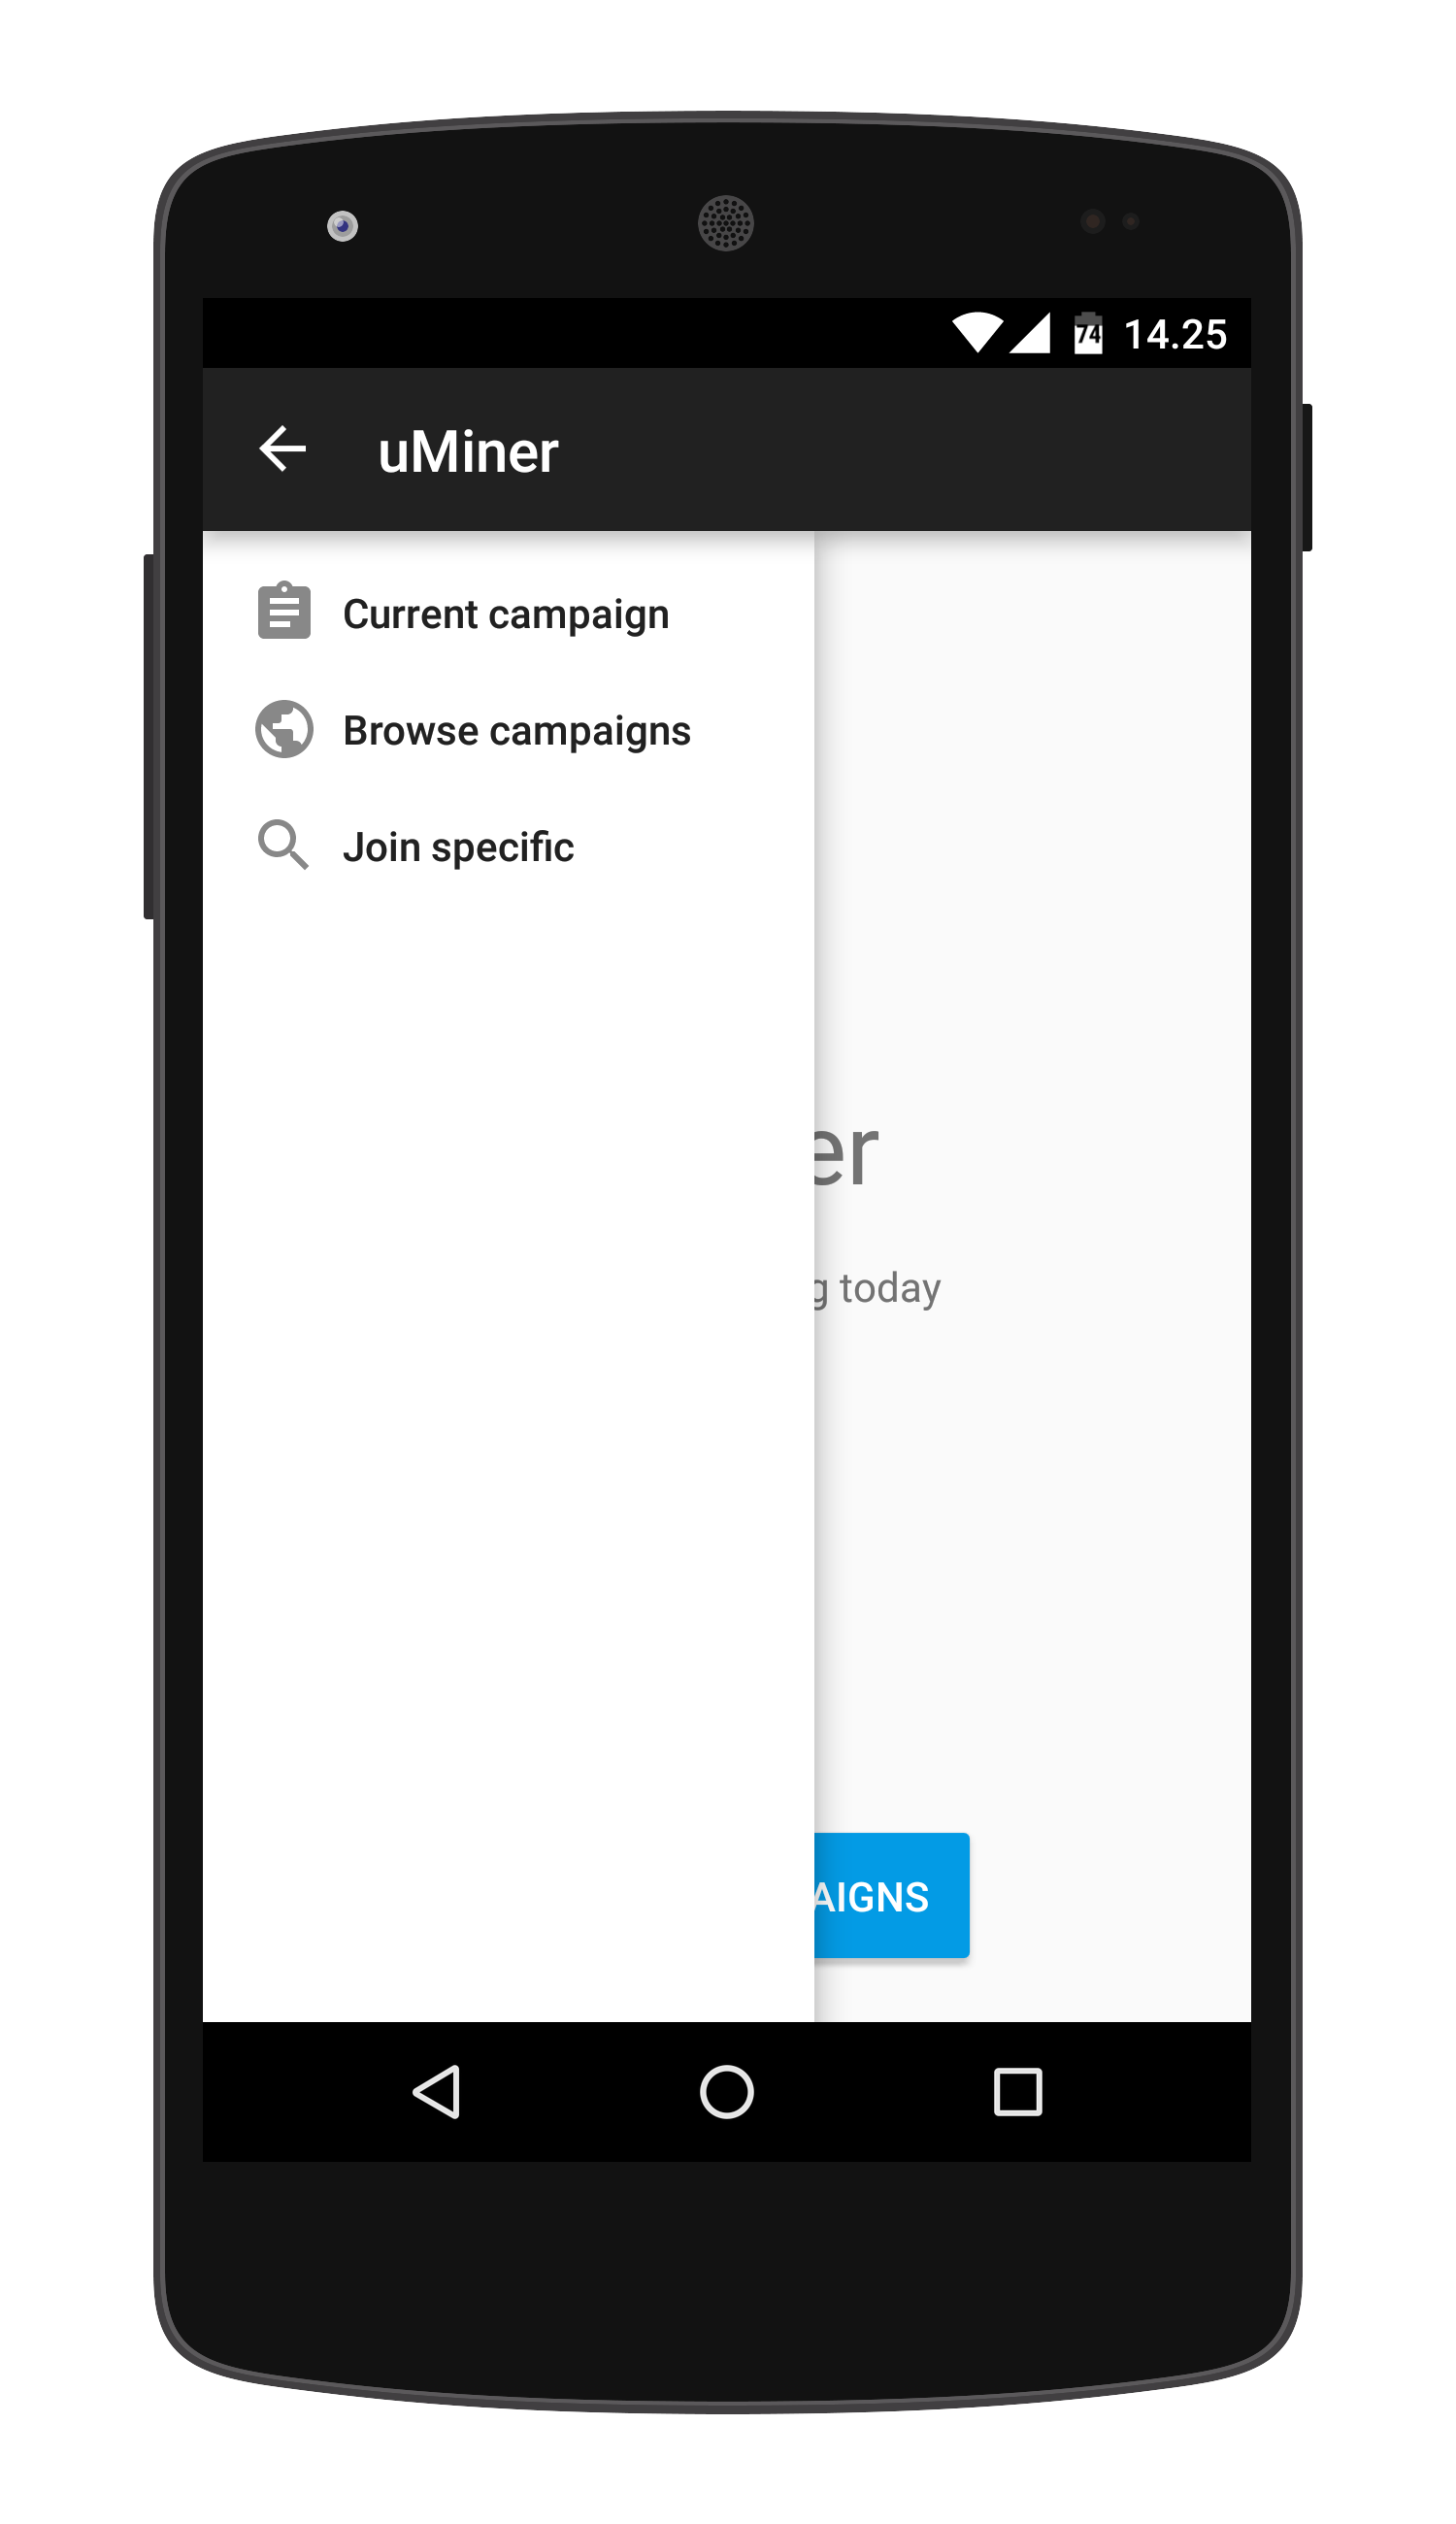
\includegraphics[width=.35\linewidth]{user_interfaces/client/client_drawer_menu_with_phone}
    \caption{Navigation through the application.}
    \label{fig:navigation}
\end{figure}
\FloatBarrier

\subsection{Browsing Campaigns}
\label{sub:browsing_campaigns}

If a participant wants to contribute to a campaign, they may browse the publicly available campaigns. This can be done through the view seen in \figref{fig:public_campaigns}. In this view, all the campaigns listed displays the title alongside with the creator of the campaign. If the participant wishes to know more about one of the listed campaign, he/she can press on that campaign and be redirected to a view similar to the one seen in \figref{fig:campaign_specification}. 

% Publicly available campaigns
\begin{figure}[!htbp]
    \begin{subfigure}[!t]{.48\textwidth}
        \centering
        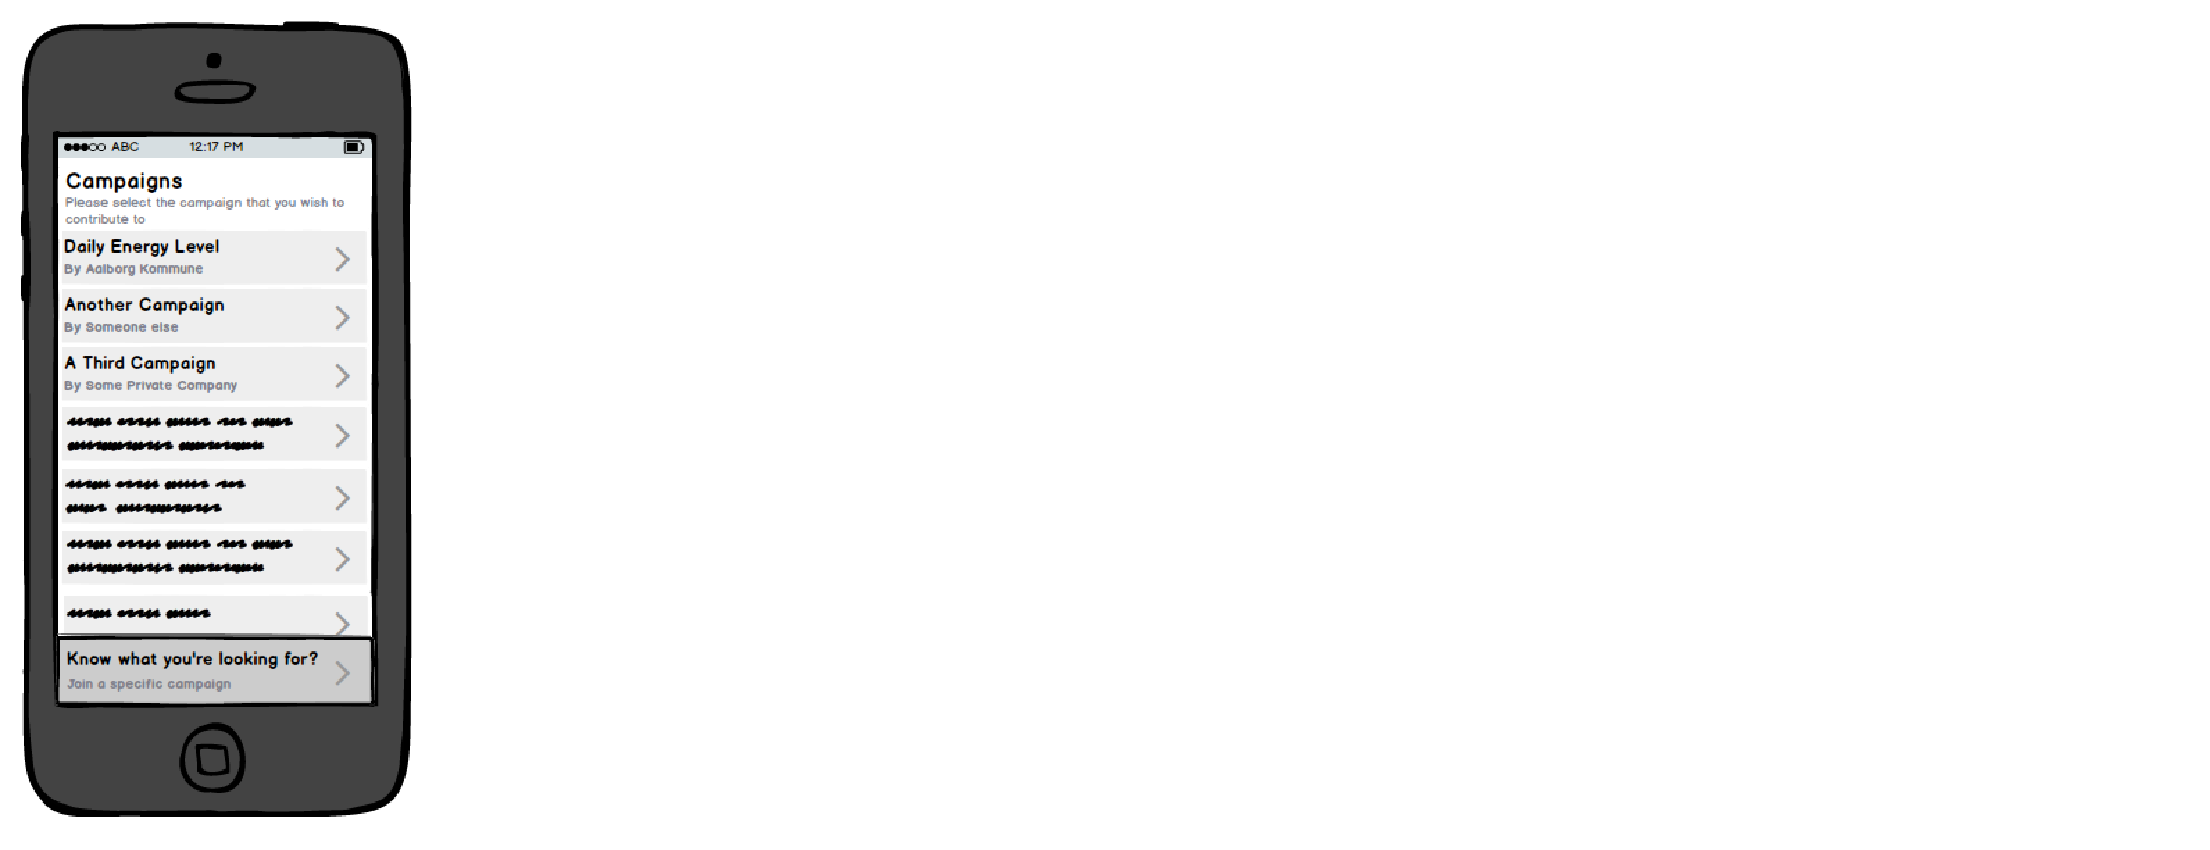
\includegraphics[width=.7\linewidth]{mockups/campaigns_list}
        \caption{Mockup of the browsing view.}
        \label{fig:mockup_public_campaigns}
    \end{subfigure}%
    \begin{subfigure}[!t]{.52\textwidth}
        \centering
        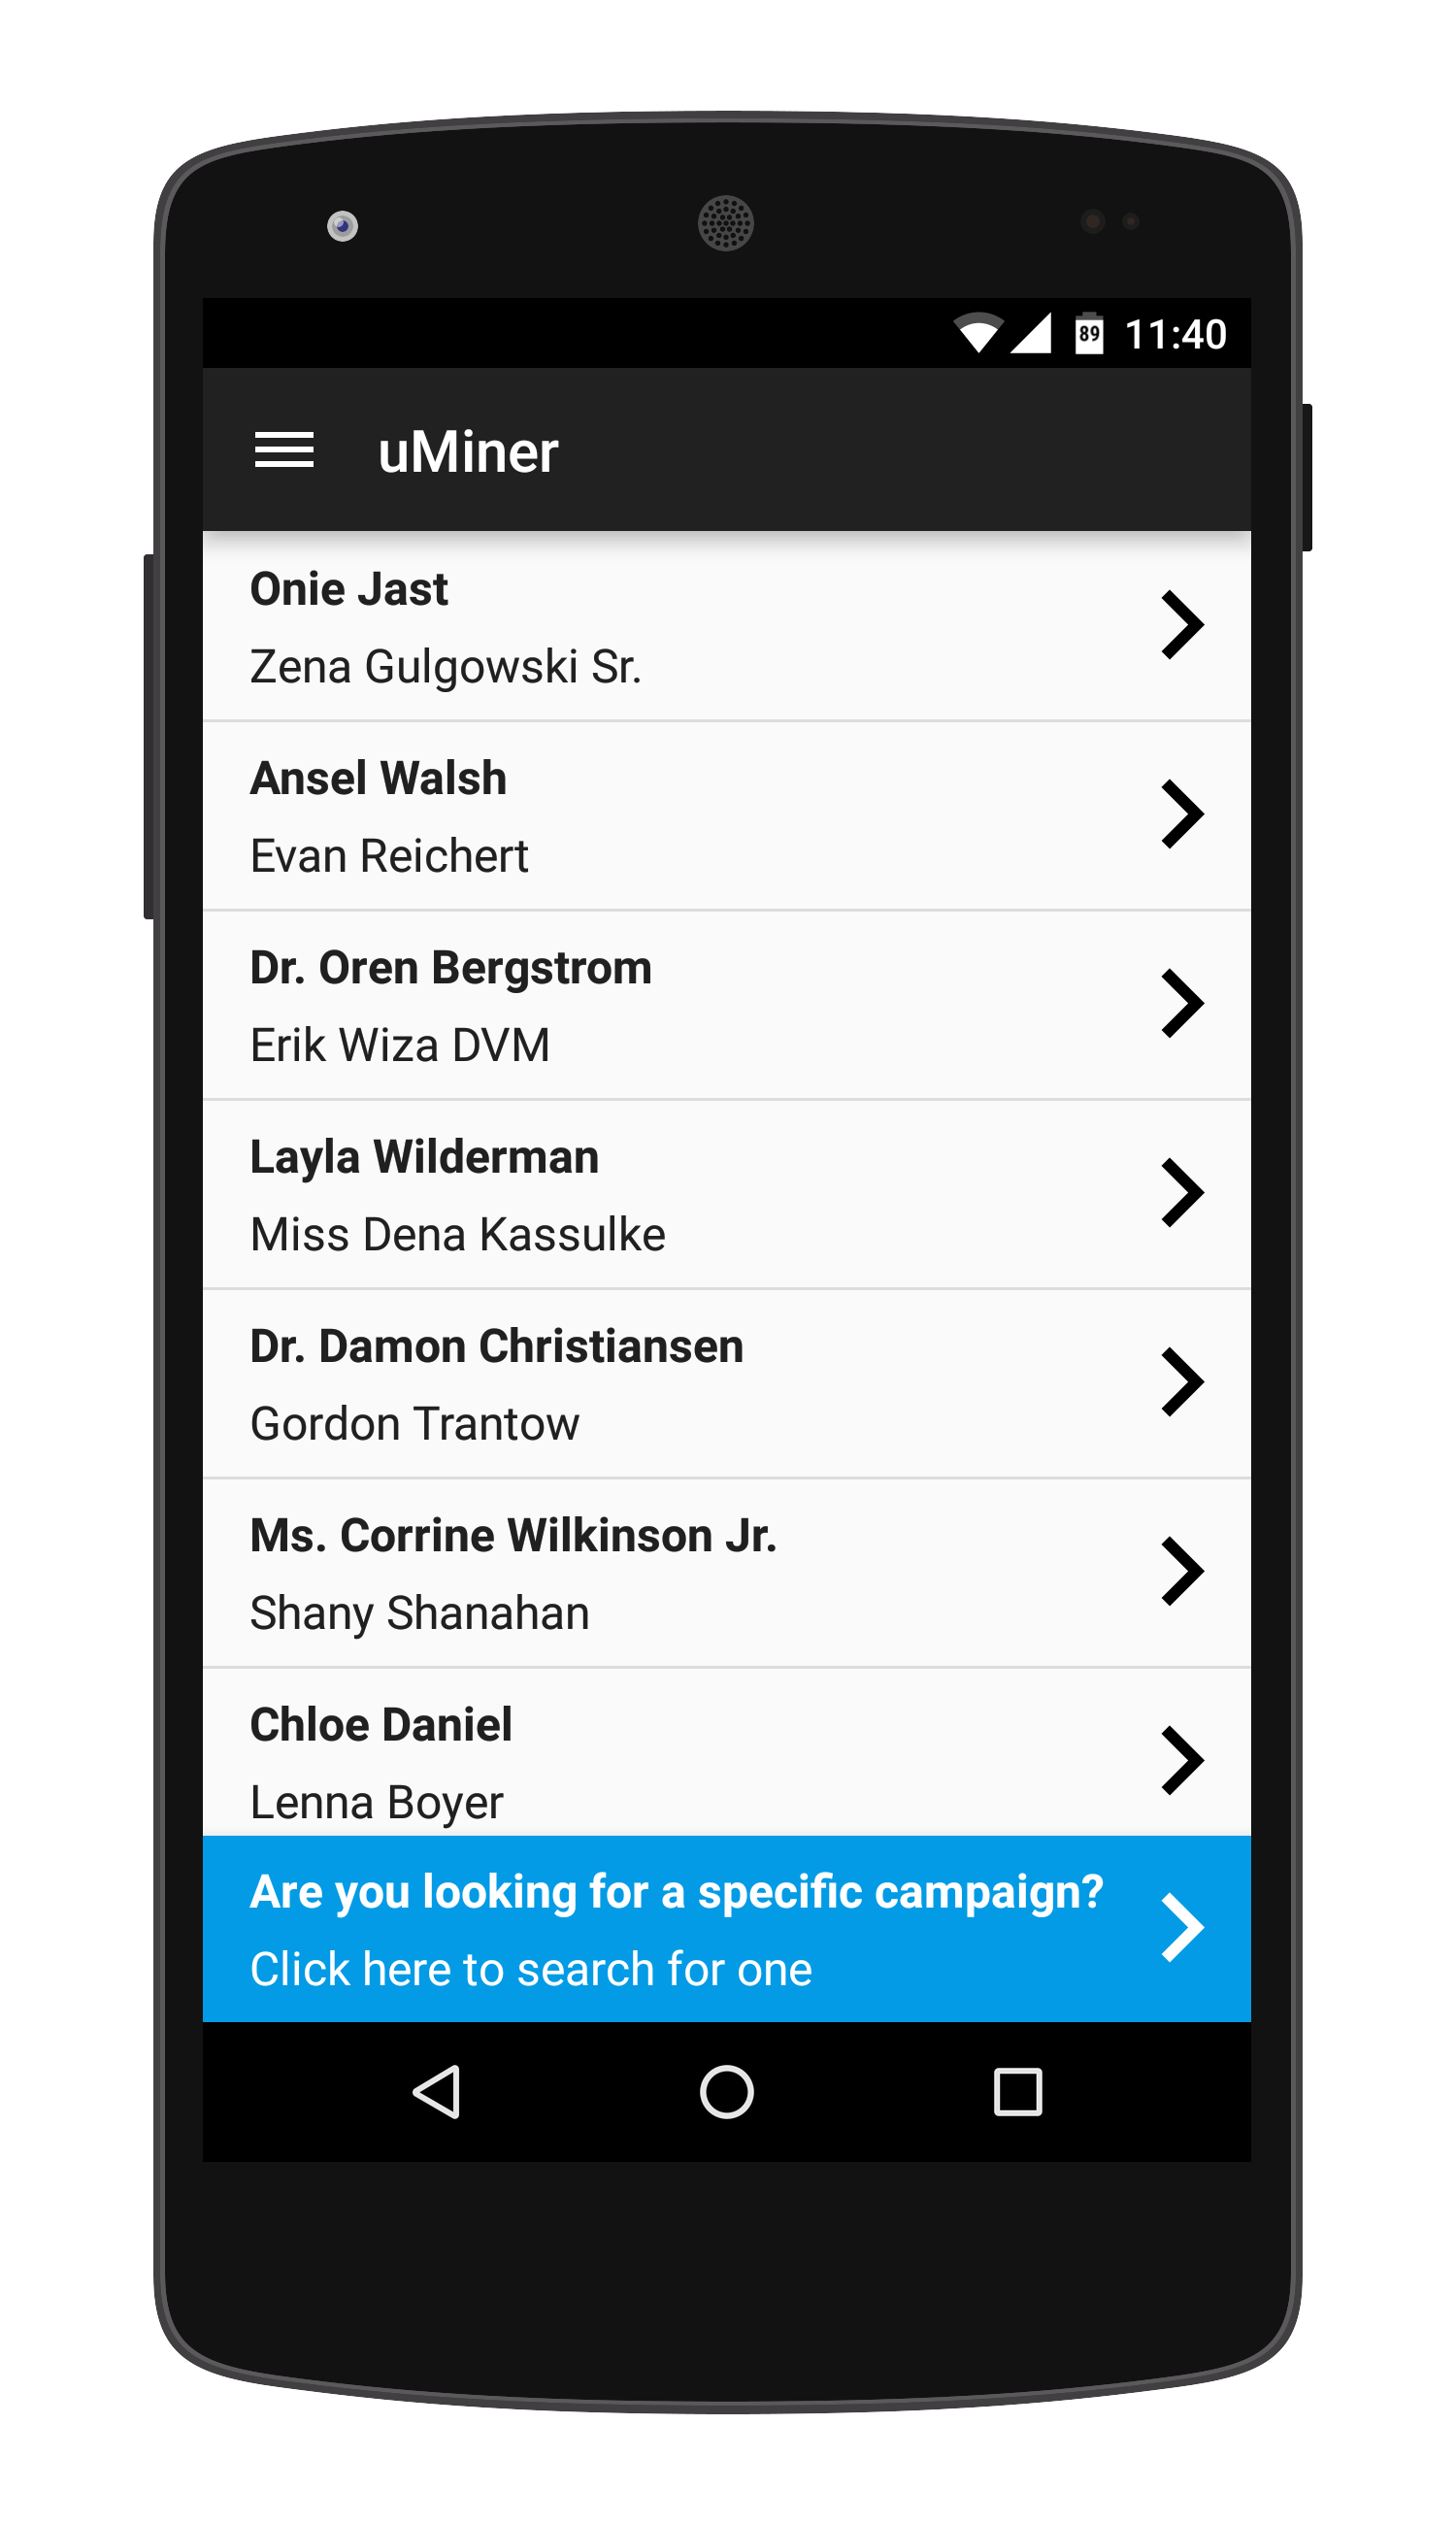
\includegraphics[width=.73\linewidth]{user_interfaces/client/client_public_campaigns_with_phone}
        \caption{Implementation of the browsing view.}
        \label{fig:implementation_public_campaigns}
    \end{subfigure}
    \caption{Mockup and implementation of browsing campaigns.}
    \label{fig:public_campaigns}
\end{figure}
\FloatBarrier

In the browsing view the participant also has the opportunity to join a specific campaign by pressing the bottom-most blue button (join specific button), which will always be visible regardless of how far the participant scroll in the list. If the participant presses on the join specific button he/she will be redirected to the view showed in \figref{fig:specific_campaign}. Here participants can enter a unique campaign identifier. If the identifier corresponds to a campaign, the participant will be redirected to a view similar to the one seen in \figref{fig:campaign_specification}. If not, he/she will be notified that the entered campaign identifier is invalid, explanation of how to know what the identifier is, can be seen in \secref{sec:customer_interaction}. 

% Search for a campaign through a campaign identifier
\begin{figure}[!htbp]
    \begin{subfigure}[!t]{.48\textwidth}
        \centering
        
\includegraphics[width=.7\linewidth]{mockups/join_specific_campaign}
        \caption{Mockup for the searching.}
        \label{fig:mockup_specific_campaign}
    \end{subfigure}%
    \begin{subfigure}[!t]{.52\textwidth}
        \centering
        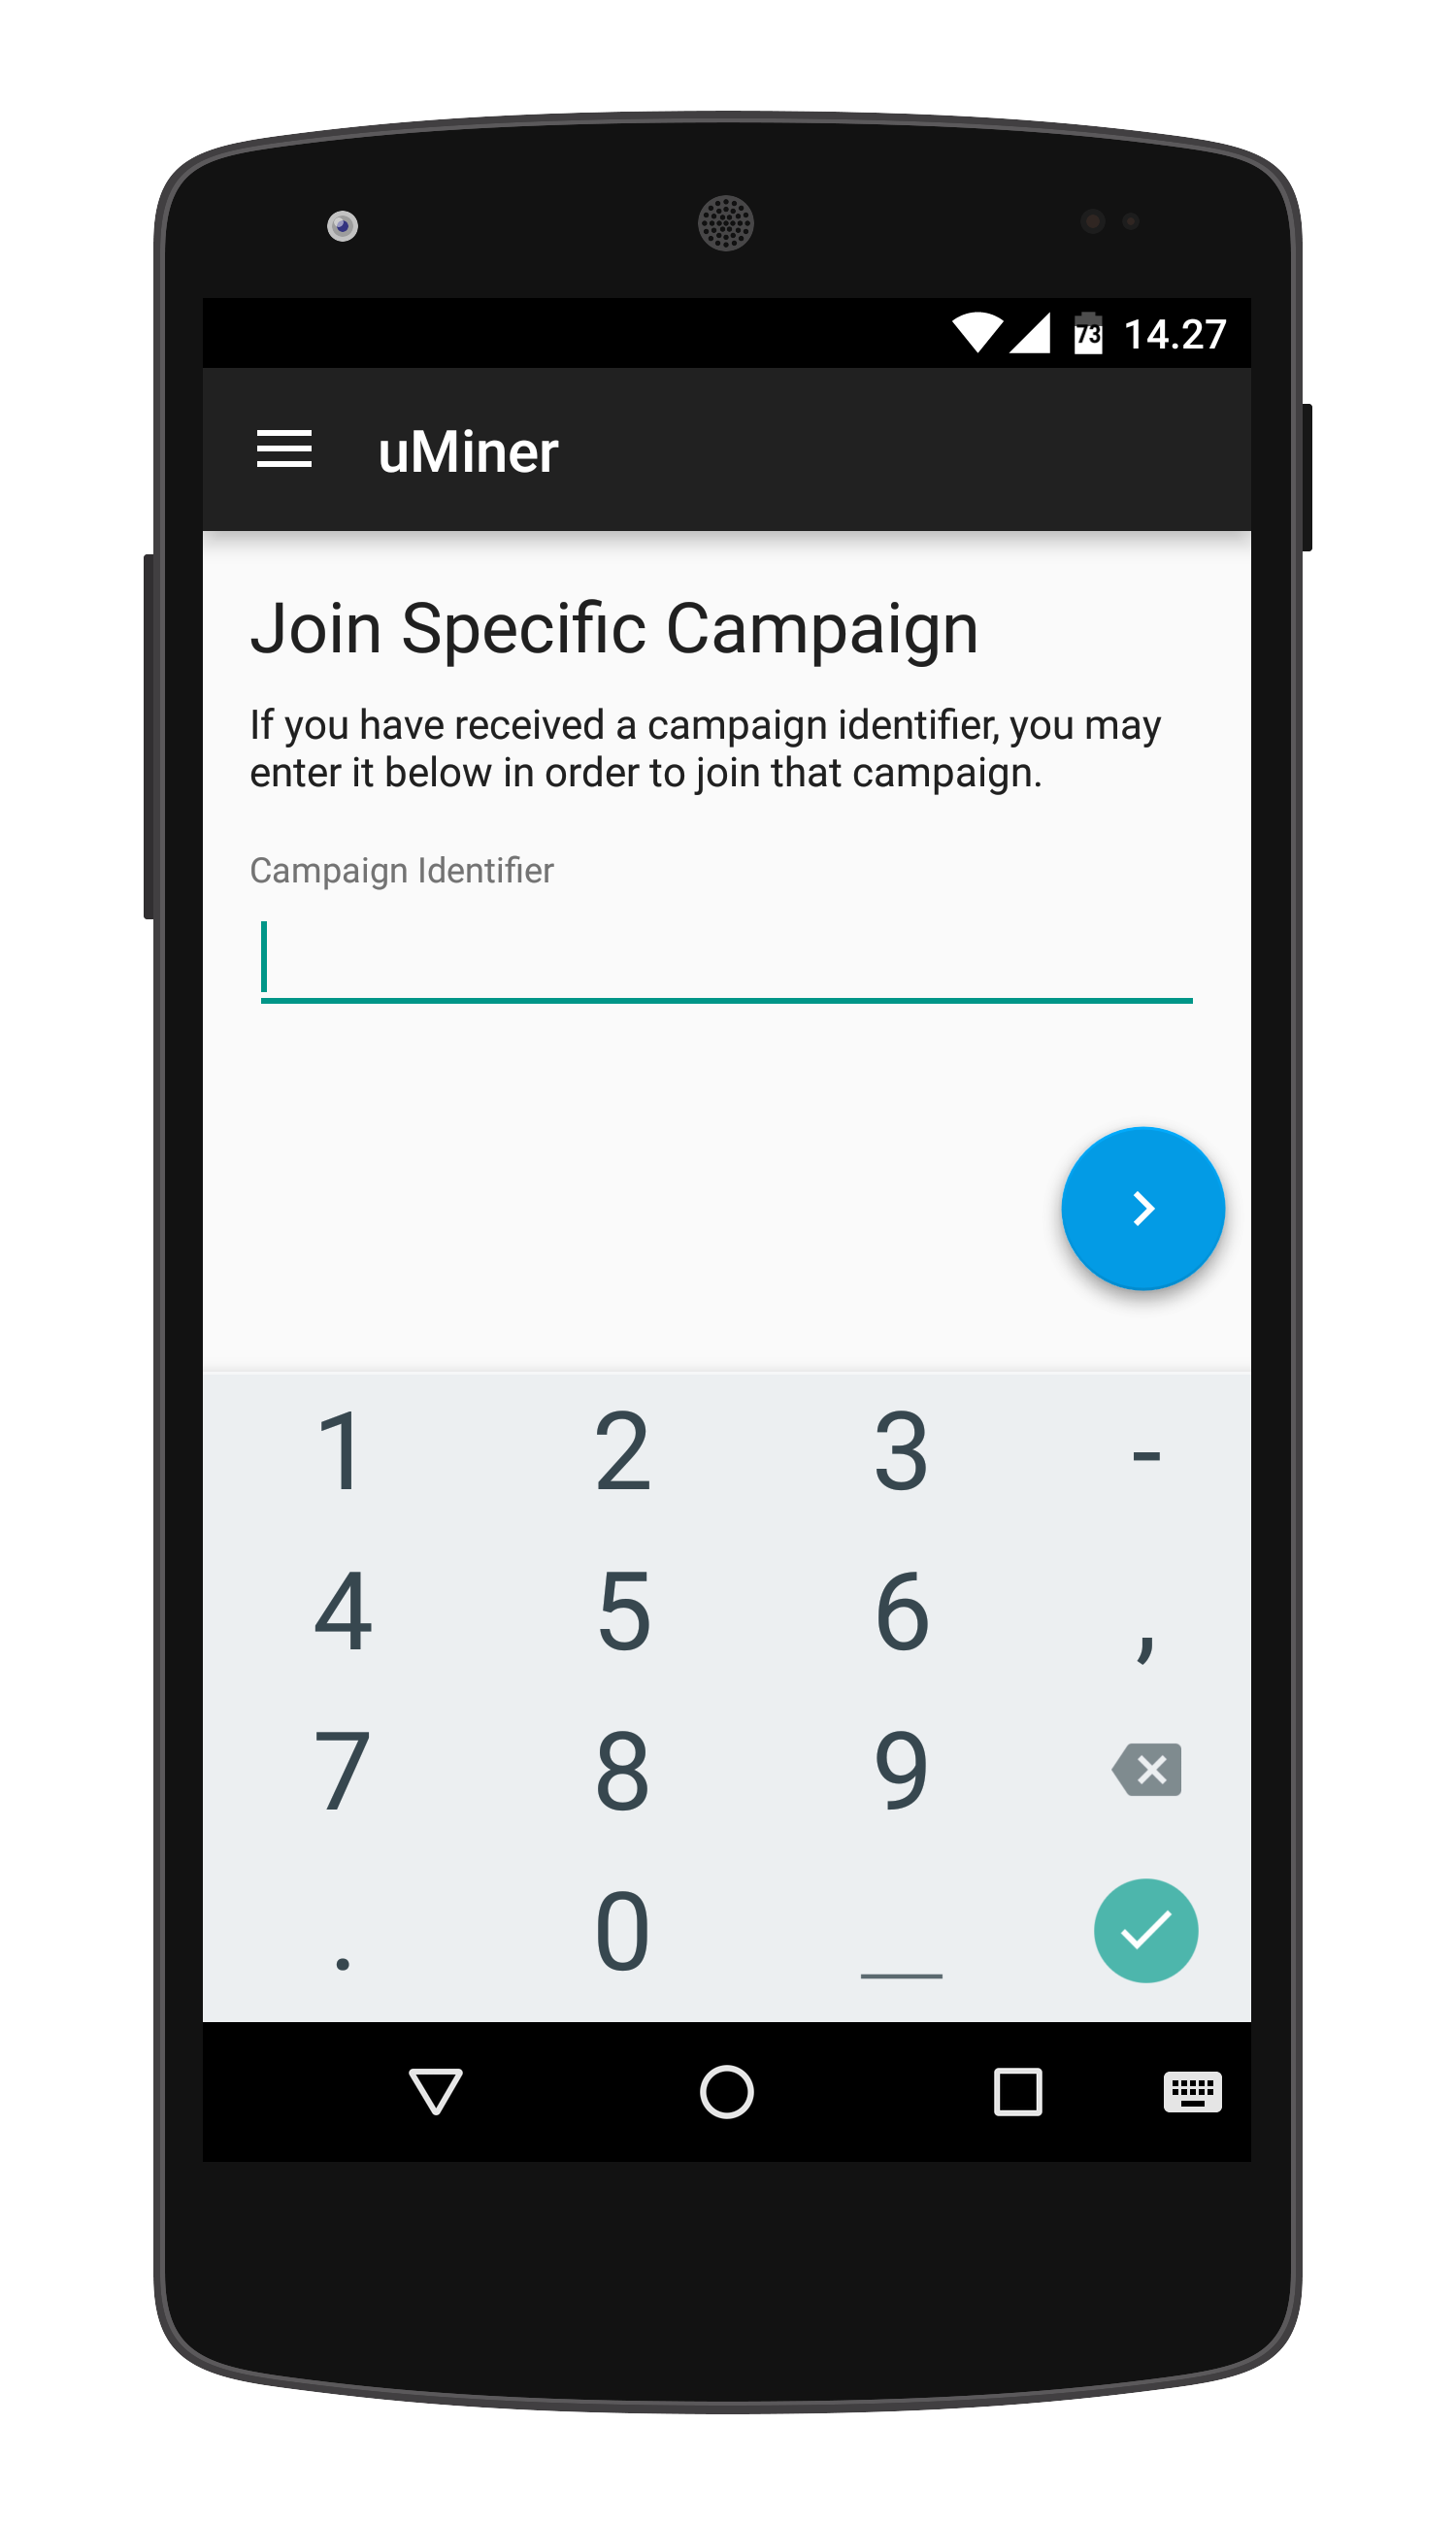
\includegraphics[width=.73\linewidth]{user_interfaces/client/client_join_specific_campaign_with_phone}
        \caption{Implementation for the searching.}
        \label{fig:implementation_specific_campaign}
    \end{subfigure}
    \caption{Mockup and Implementation for searching for a specific campaign using a campaign identifier.}
    \label{fig:specific_campaign}
\end{figure}
\FloatBarrier

Throughout the project, we have thought of quite a number of different ways of allowing the participants to search for campaigns using different search criteria:

\begin{description}
    \item[Quick Response (QR) Code] could be utilized to give participants an easy way of subscribing to campaigns, by scanning a QR code. Customers would be able to distribute these QR codes through both digital and printed media. Furthermore, QR codes might be more easily relatable for participants, since they might be familiar with the concept from other domains.

    \item[Specific search criteria] might help participants to find exactly what they want to contribute to. Participants might only want to contribute to campaigns with a scientific background, or campaigns that have next to no impact on battery life. Other criteria might be: limited amount of, or no questions, in questionnaires. Additionally, some participants might not be willing to contribute to campaigns with specific sensors, e.g. GPS, so the possibility of searching for campaigns with specific search criteria might be desirable.

    \item[Prizes and other motivational factors] will potentially have a big impact on which campaigns gets contributed to. This means that the application could assist customers in getting more participants for their campaigns by displaying information regarding the prizes that customers might provide to willing participants. One could also imagine that participants could filter campaigns with or without prizes.
\end{description} 

\subsection{Contributing to Campaigns}
\label{sub:contributing_to_campaigns}

To contribute to a specific campaign, participants must first find a campaign that the want to contribute to. This can be done through the campaign browser, previously shown in \figref{fig:public_campaigns}, or entering a unique identifier in the join specific campaign view, previously shown in \figref{fig:specific_campaign}. The participants must then navigate to a campaign specification view, similar to the one seen in \figref{fig:campaign_specification}. Here, participants can view the details of the campaign; after reviewing this information, they can then decide if they want to contribute by subscribing to the campaign, which will be done by pressing the green subscribe button. This will start the gathering process, and how this process works is described in \charef{cha:gathering_sensor_data}\todo{overvej om denne ref skal være til en specific sektion i stedet for hele kapitlet}.

% Campaign specification
\begin{figure}[!htbp]
    \begin{subfigure}[!t]{.48\textwidth}
        \centering
        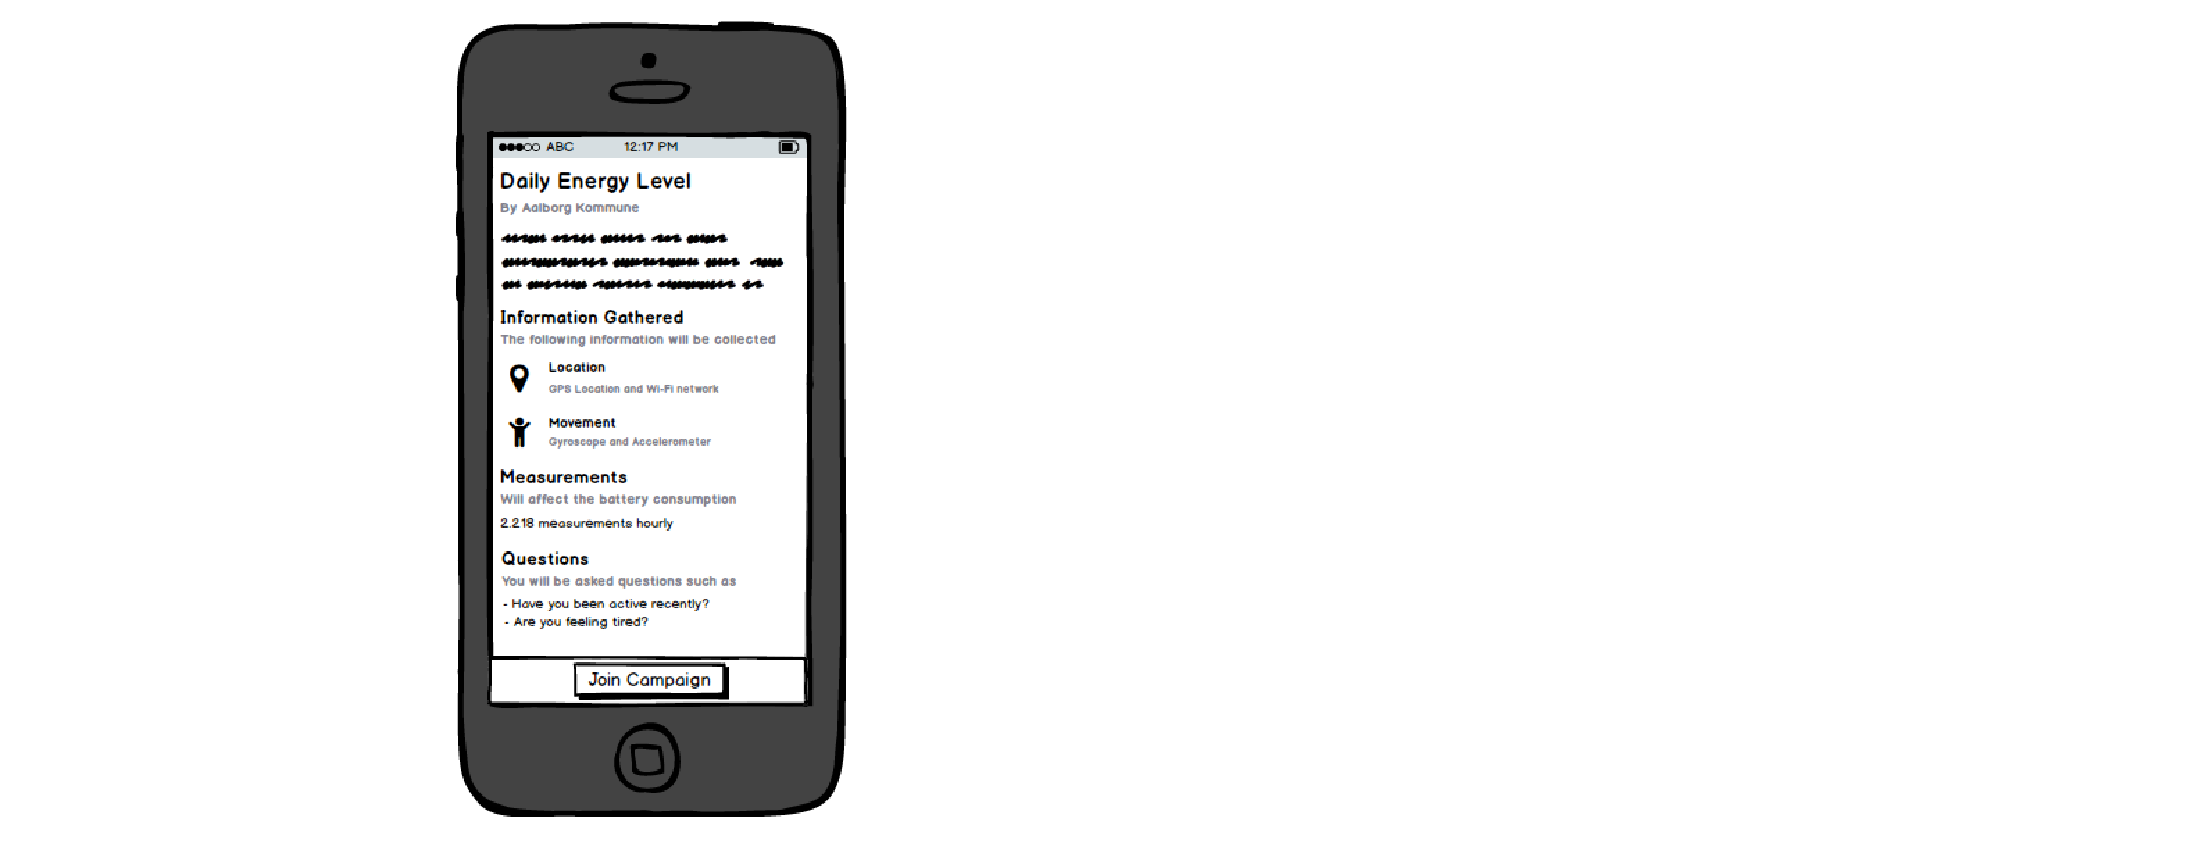
\includegraphics[width=.7\linewidth]{mockups/campaign_specification}
        \caption{Mockup of the specification.}
        \label{fig:mockup_campaign_specification}
    \end{subfigure}%
    \begin{subfigure}[!t]{.52\textwidth}
        \centering
        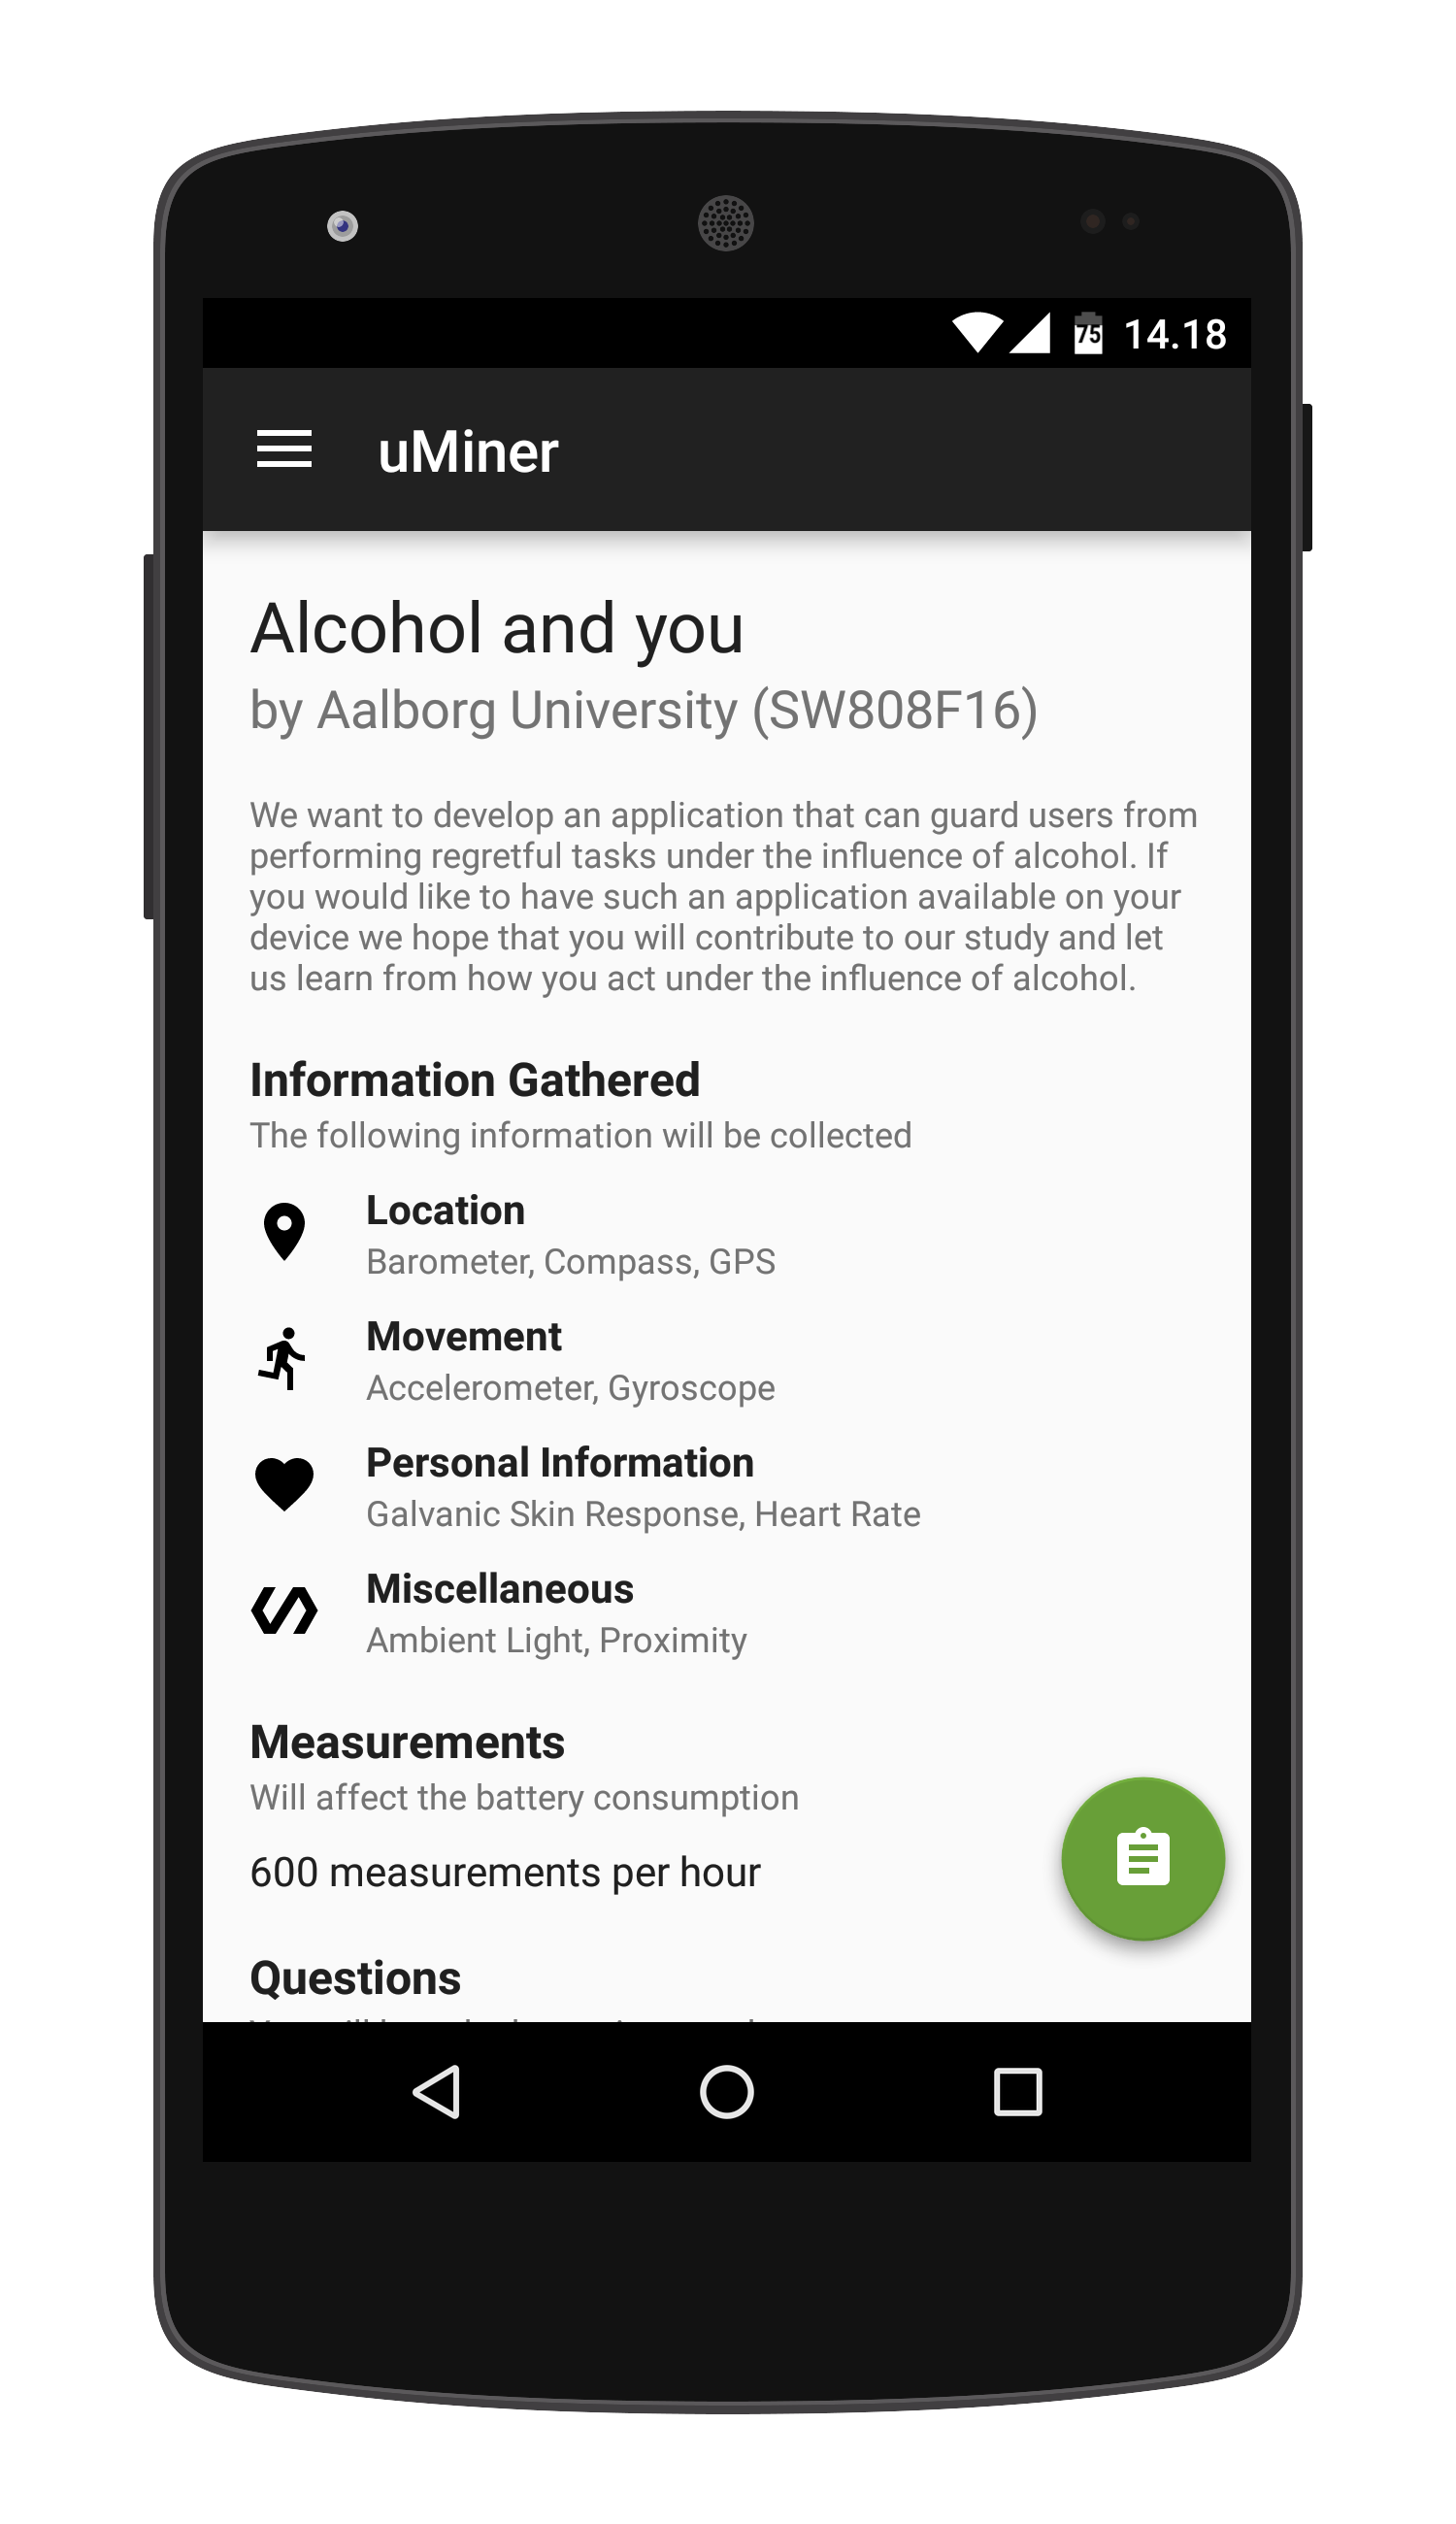
\includegraphics[width=.73\linewidth]{user_interfaces/client/client_campaign_specification2_with_phone}
        \caption{Implementation of the specification.}
        \label{fig:implementation_campaign_specification}
    \end{subfigure}
    \caption{Mockup and implementation of the specification view for a specific campaign.}
    \label{fig:campaign_specification}
\end{figure}
\FloatBarrier

If for any reason, a participant no longer wishes to contribute to the campaign he/she is subscribed to, he/she can navigate to the specification for subscribed campaign. In the specification view, the green subscribe button will instead be a red unsubscribe button, as seen in \figref{fig:leave_campaign_no_dialog}. Pressing this button, will trigger a confirmation dialog, as seen in \figref{fig:leave_campaign_dialog}. If the participant confirms this, by pressing yes, all data collection will immediately stop, however, participants may still be asked questions, depending on the campaign\todo{forklar kort hvorfor den gør det}. This comply with the way we intended the system to work regarding the participatory sensing as described in \secref{sec:human_activity_recognition}\todo{er det her godt nok?}.

% Leave campaign and dialog
\begin{figure}[!htbp]
    \begin{subfigure}[!t]{.50\textwidth}
        \centering
        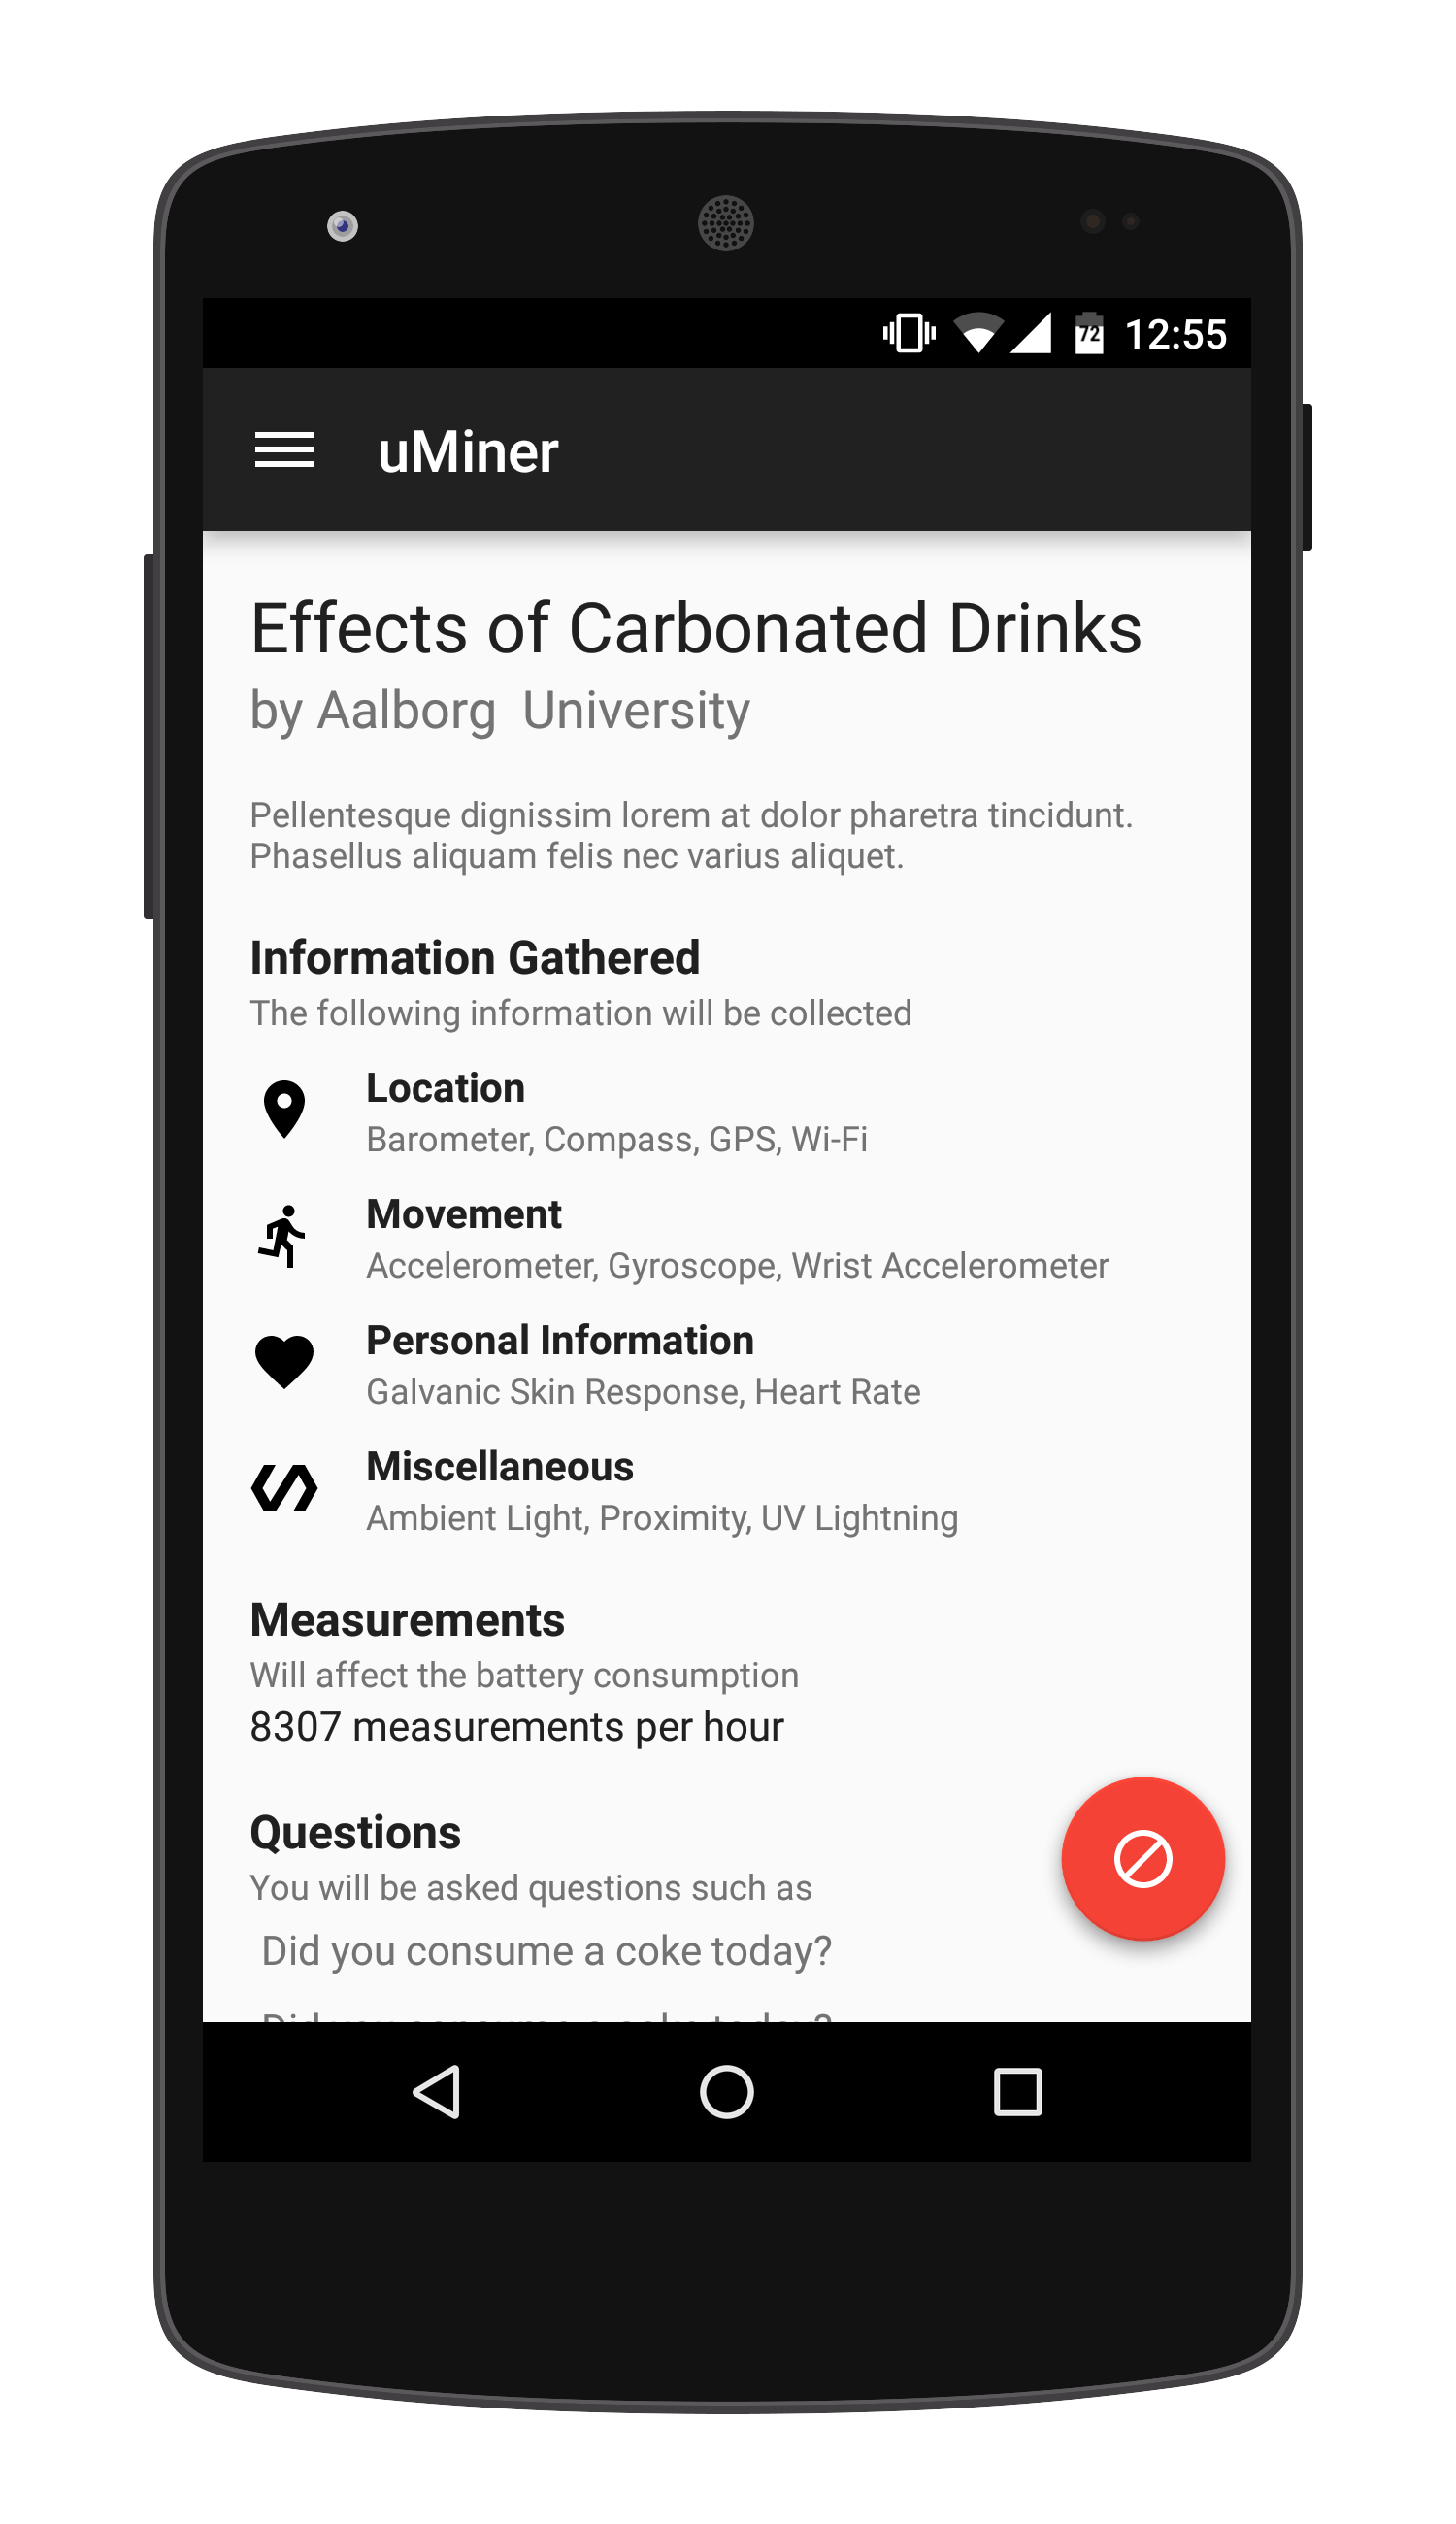
\includegraphics[width=.73\linewidth]{user_interfaces/client/client_leave_campaign_no_dialog_with_phone}
        \caption{Specification view with an unsubscribe \\\hspace{\textwidth}button.}
        \label{fig:leave_campaign_no_dialog}
    \end{subfigure}%
    \begin{subfigure}[!t]{.50\textwidth}
        \centering
        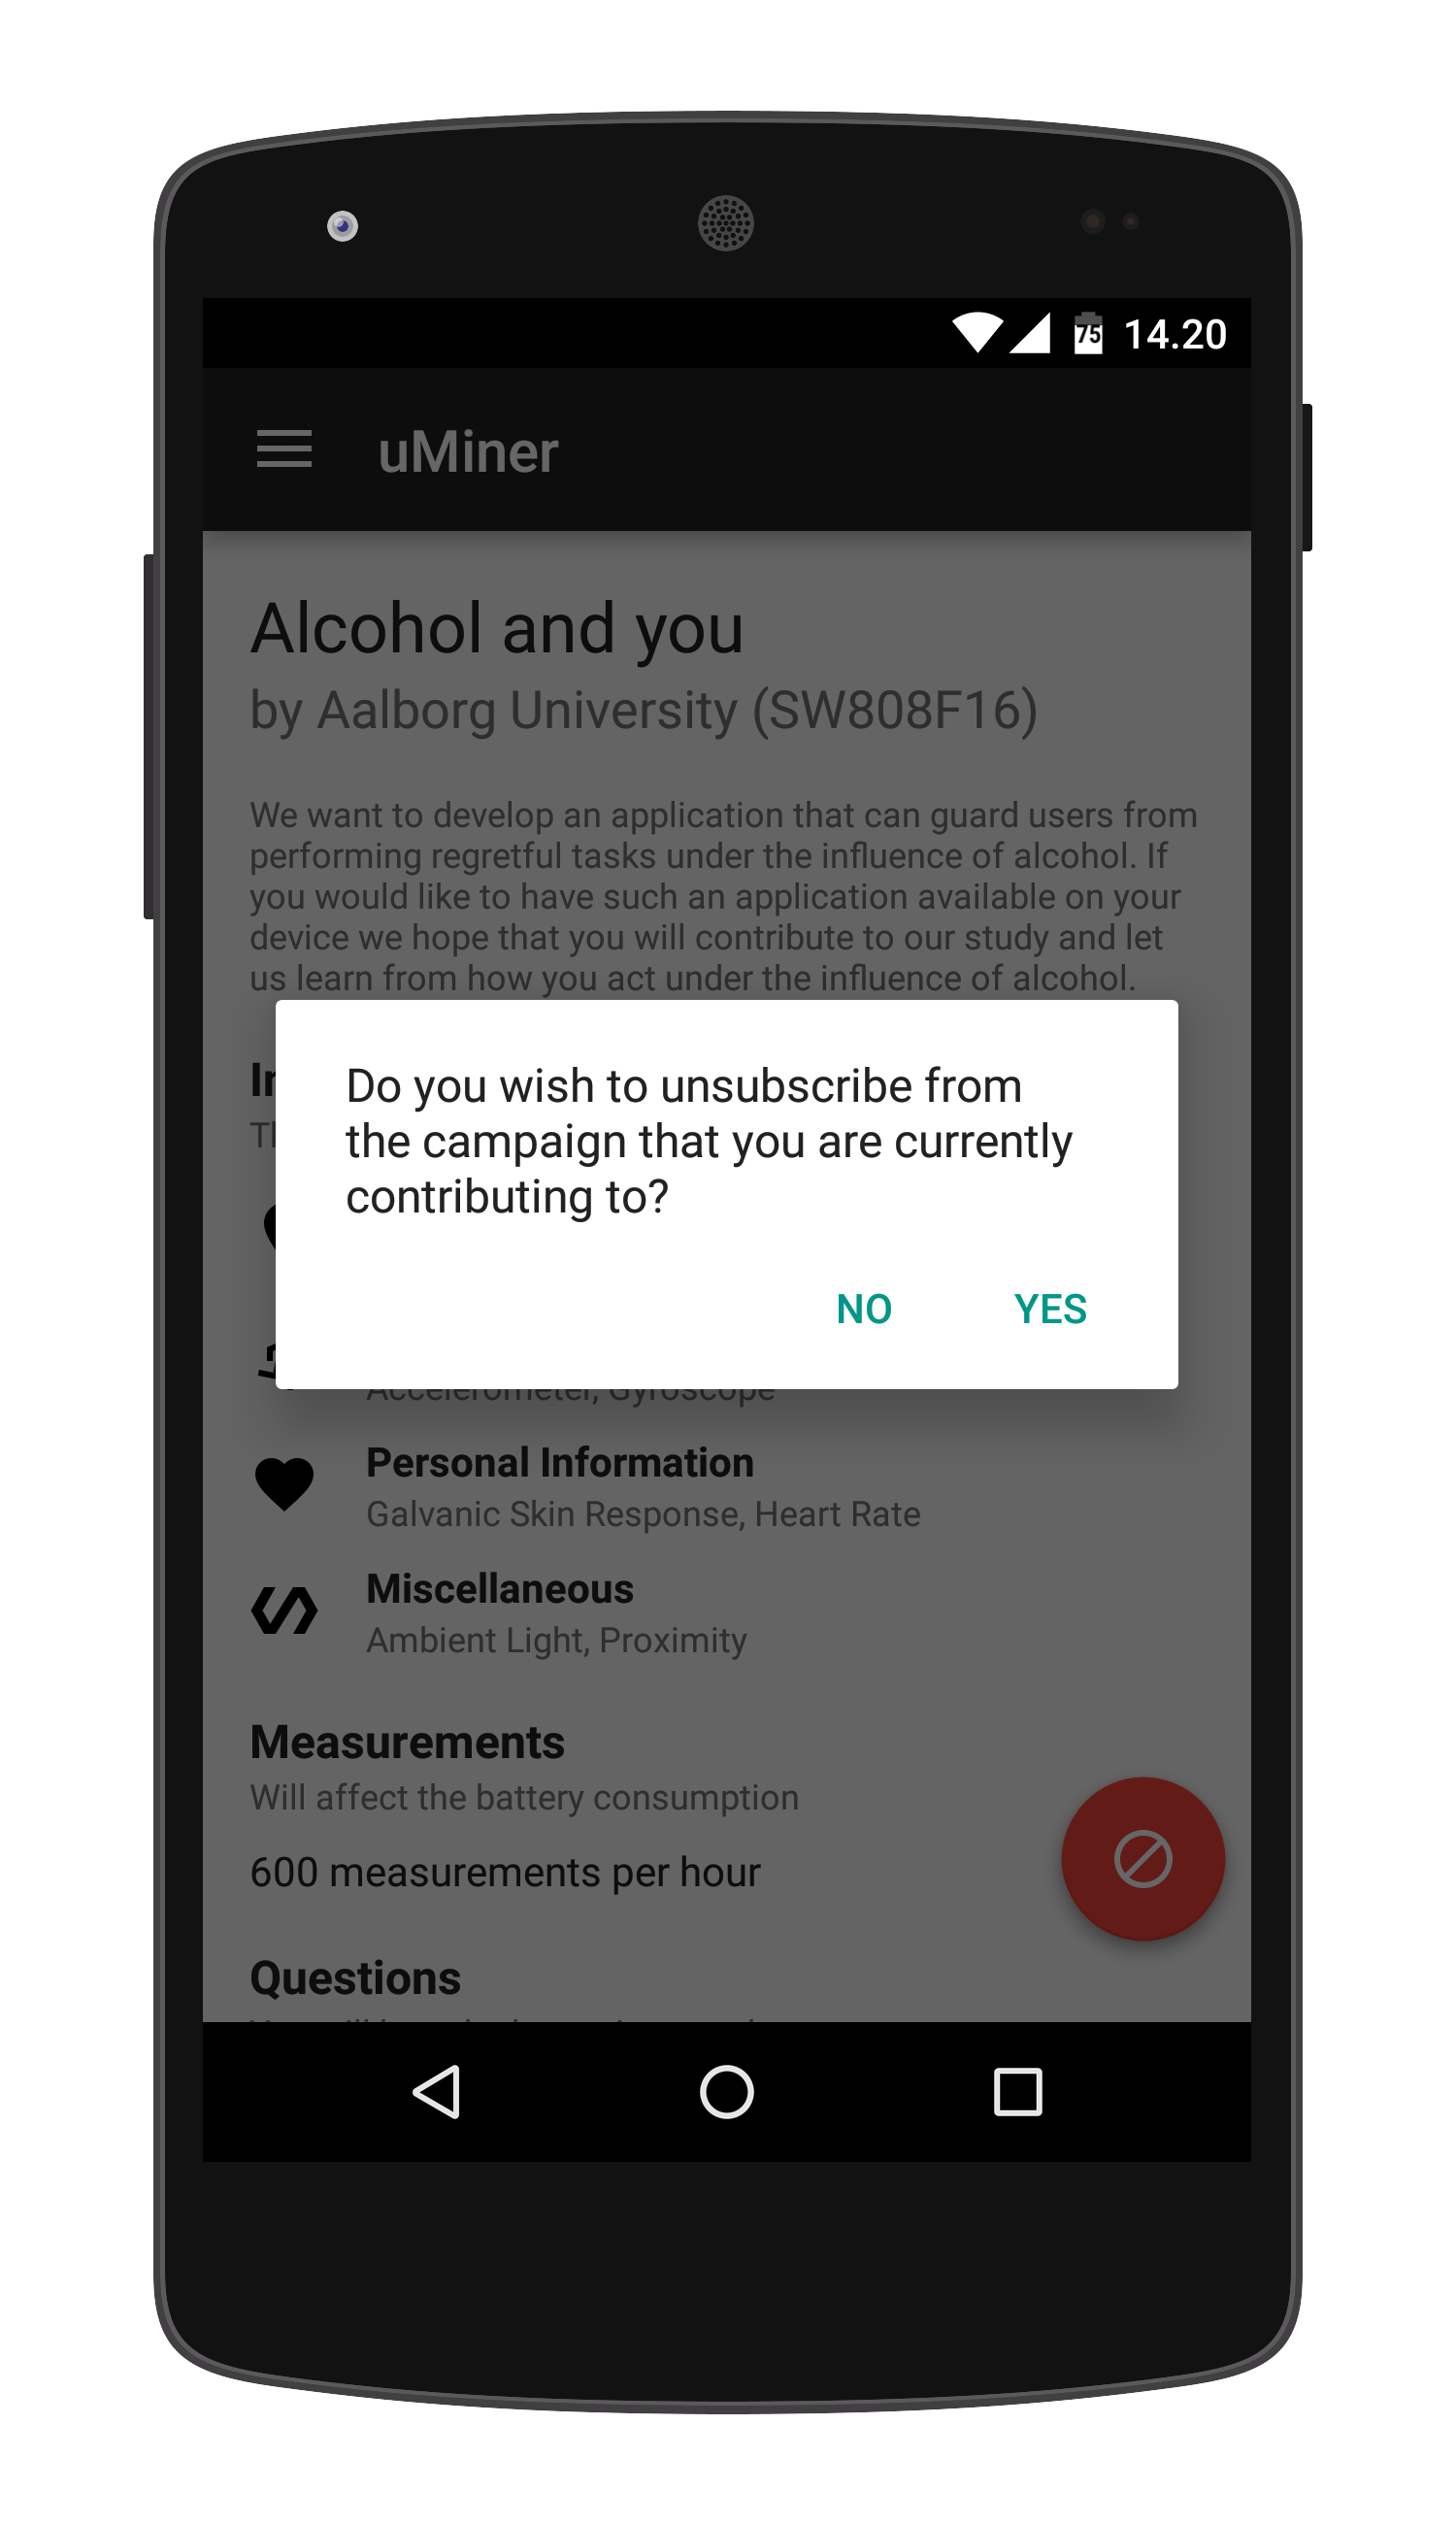
\includegraphics[width=.73\linewidth]{user_interfaces/client/client_leave_campaign_with_phone}
        \caption{Confirmation dialog triggered by pressing the unsubscribe button.}
        \label{fig:leave_campaign_dialog}
    \end{subfigure}
    \caption{Specification view of a campaign when a participant has joined a campaign.}
    \label{fig:leave_campaign}
\end{figure}
\FloatBarrier

\subsection{Answering Questionnaires}
\label{sub:answering_questionnaired}

Some campaigns might request that the participants answers a questionnaire. The request can happen when the participant has closed the application, or when the participant is not using the phone. To accompany this, we chose to use notifications to inform the participant when they should answer questionnaires, which can be seen in \figref{fig:answering_questionnaire_notification}. When the notification is pressed, the application opens with a specific activity, which can be seen in \figref{fig:answering_questionnaire_answering}. 

\todo[inline]{Overvej om at vise notifikationen hvor vores app ikke er åben}
% Answering questionnaires
\begin{figure}[!htbp]
    \begin{subfigure}[!t]{.50\textwidth}
        \centering
        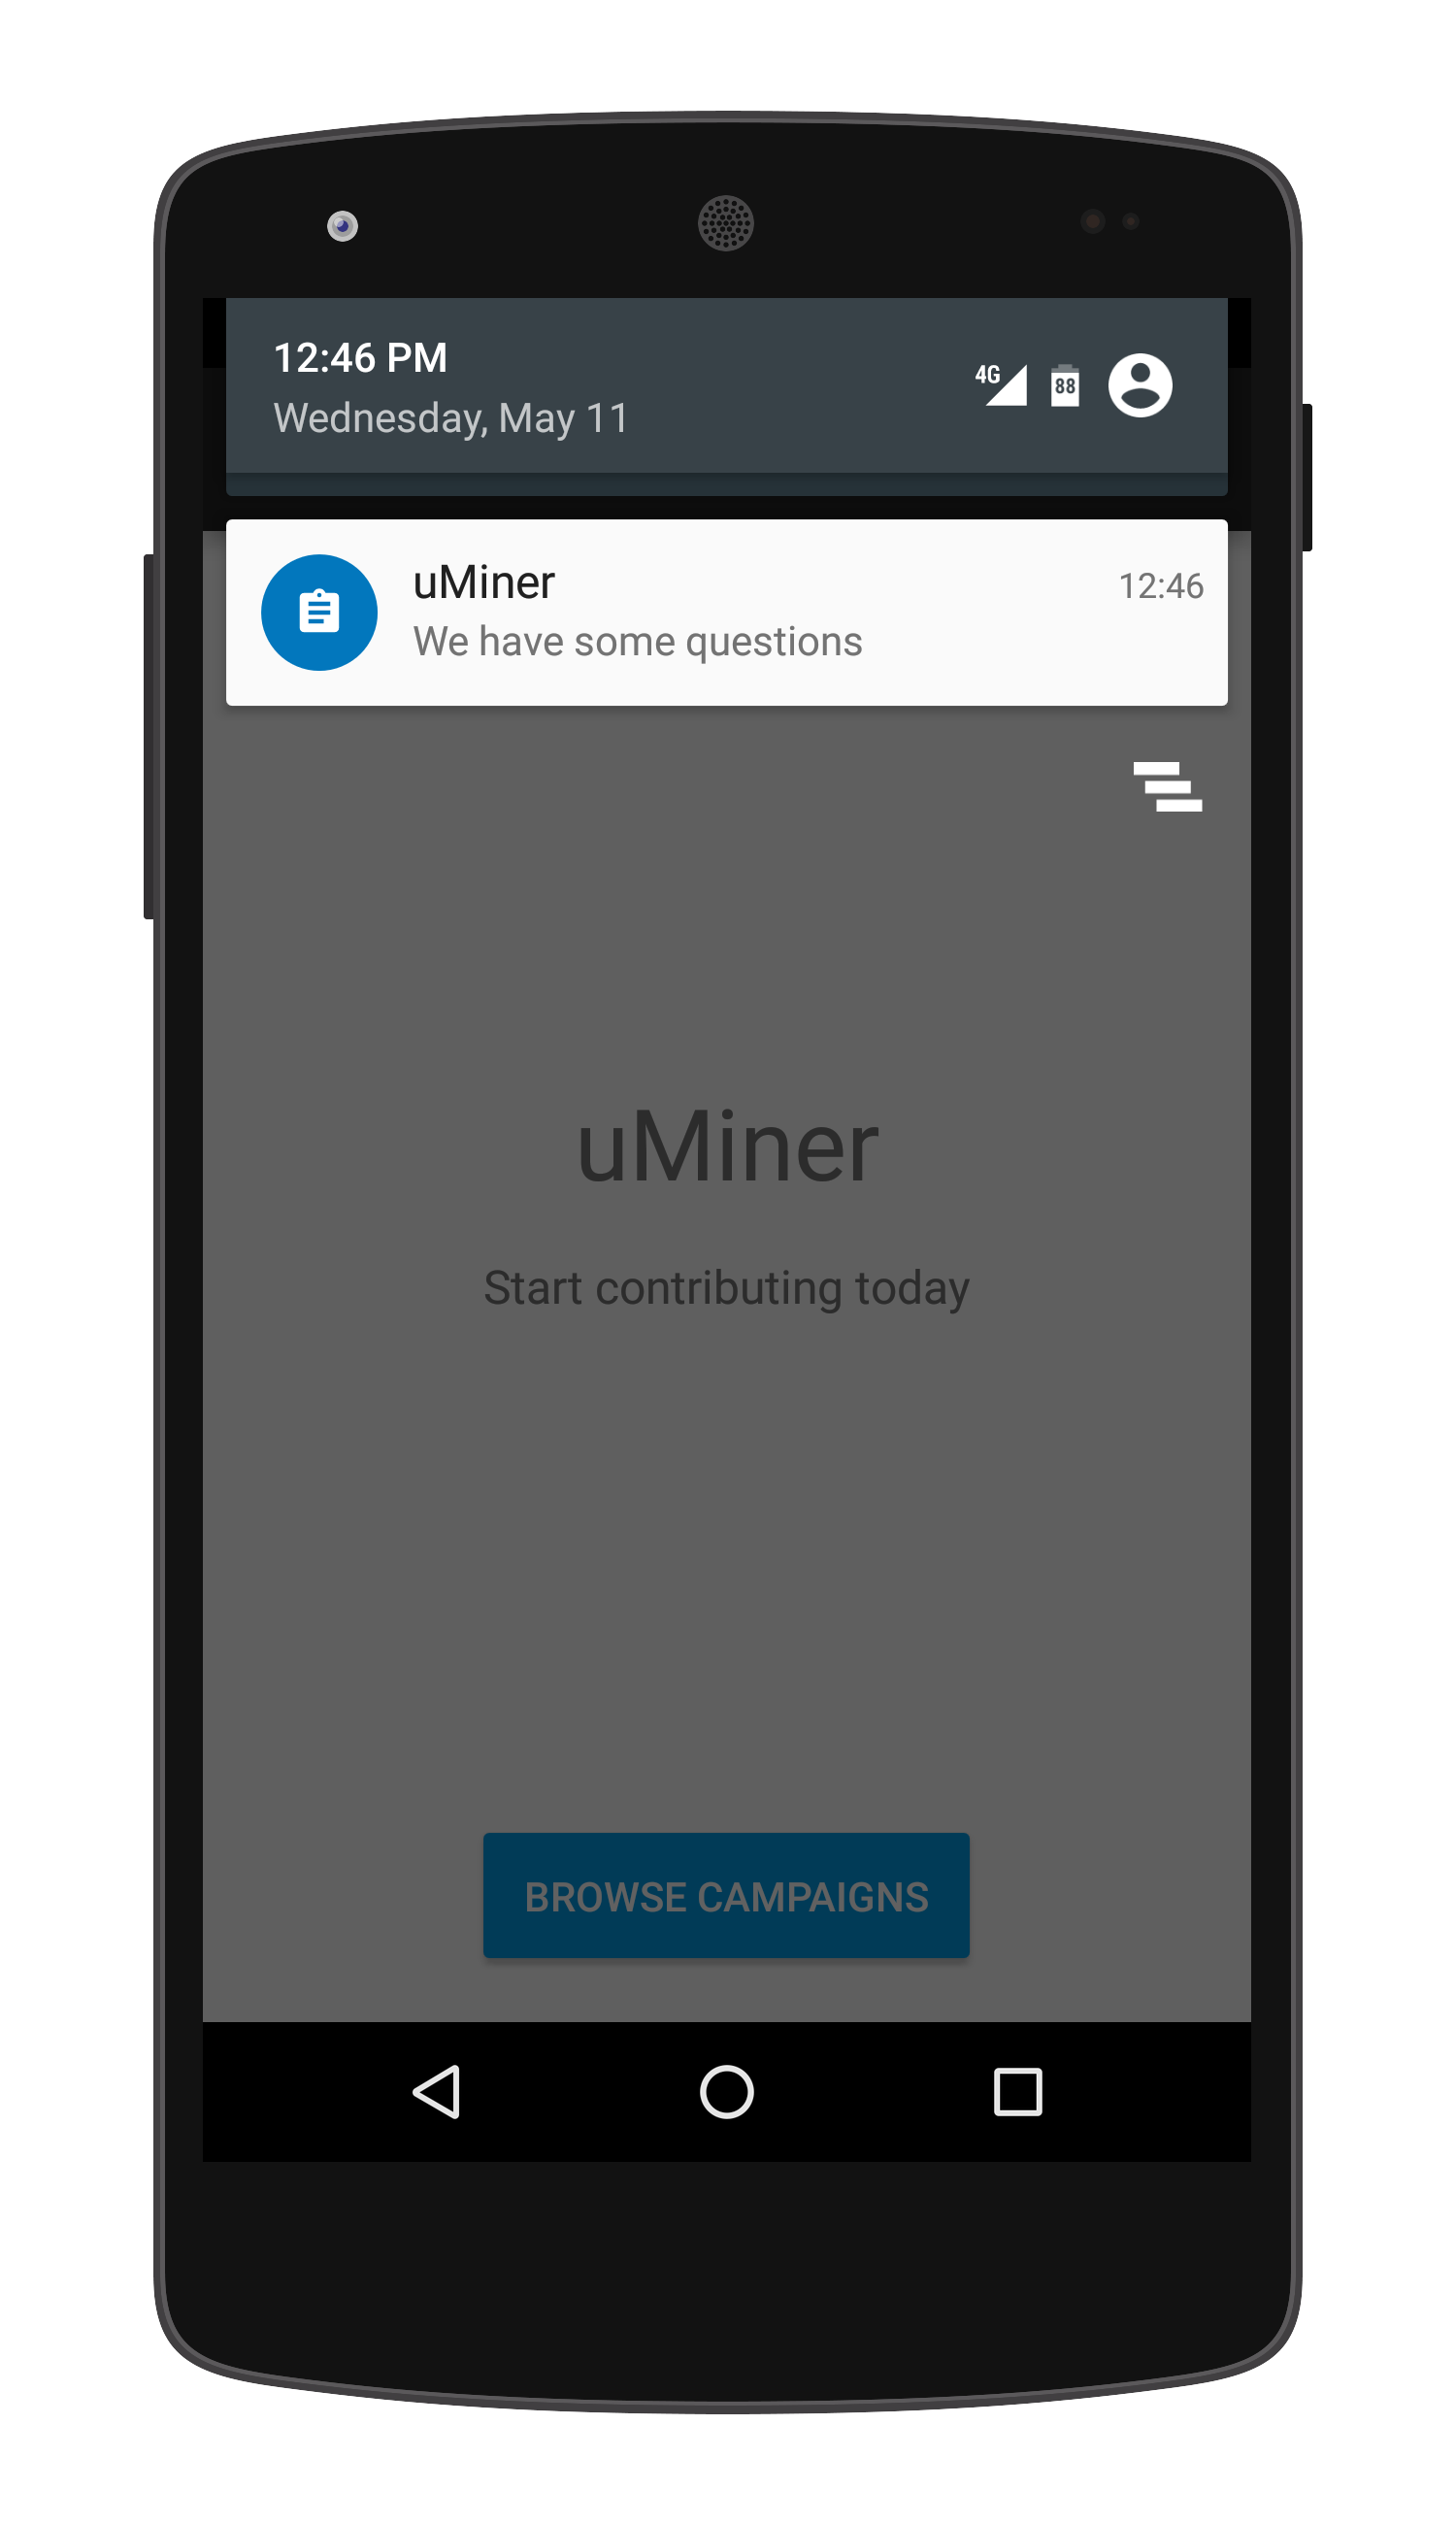
\includegraphics[width=.73\linewidth]{user_interfaces/client/client_notification_with_phone}
        \caption{Notification to answer questions.}
        \label{fig:answering_questionnaire_notification}
    \end{subfigure}%
    \begin{subfigure}[!t]{.50\textwidth}
        \centering
        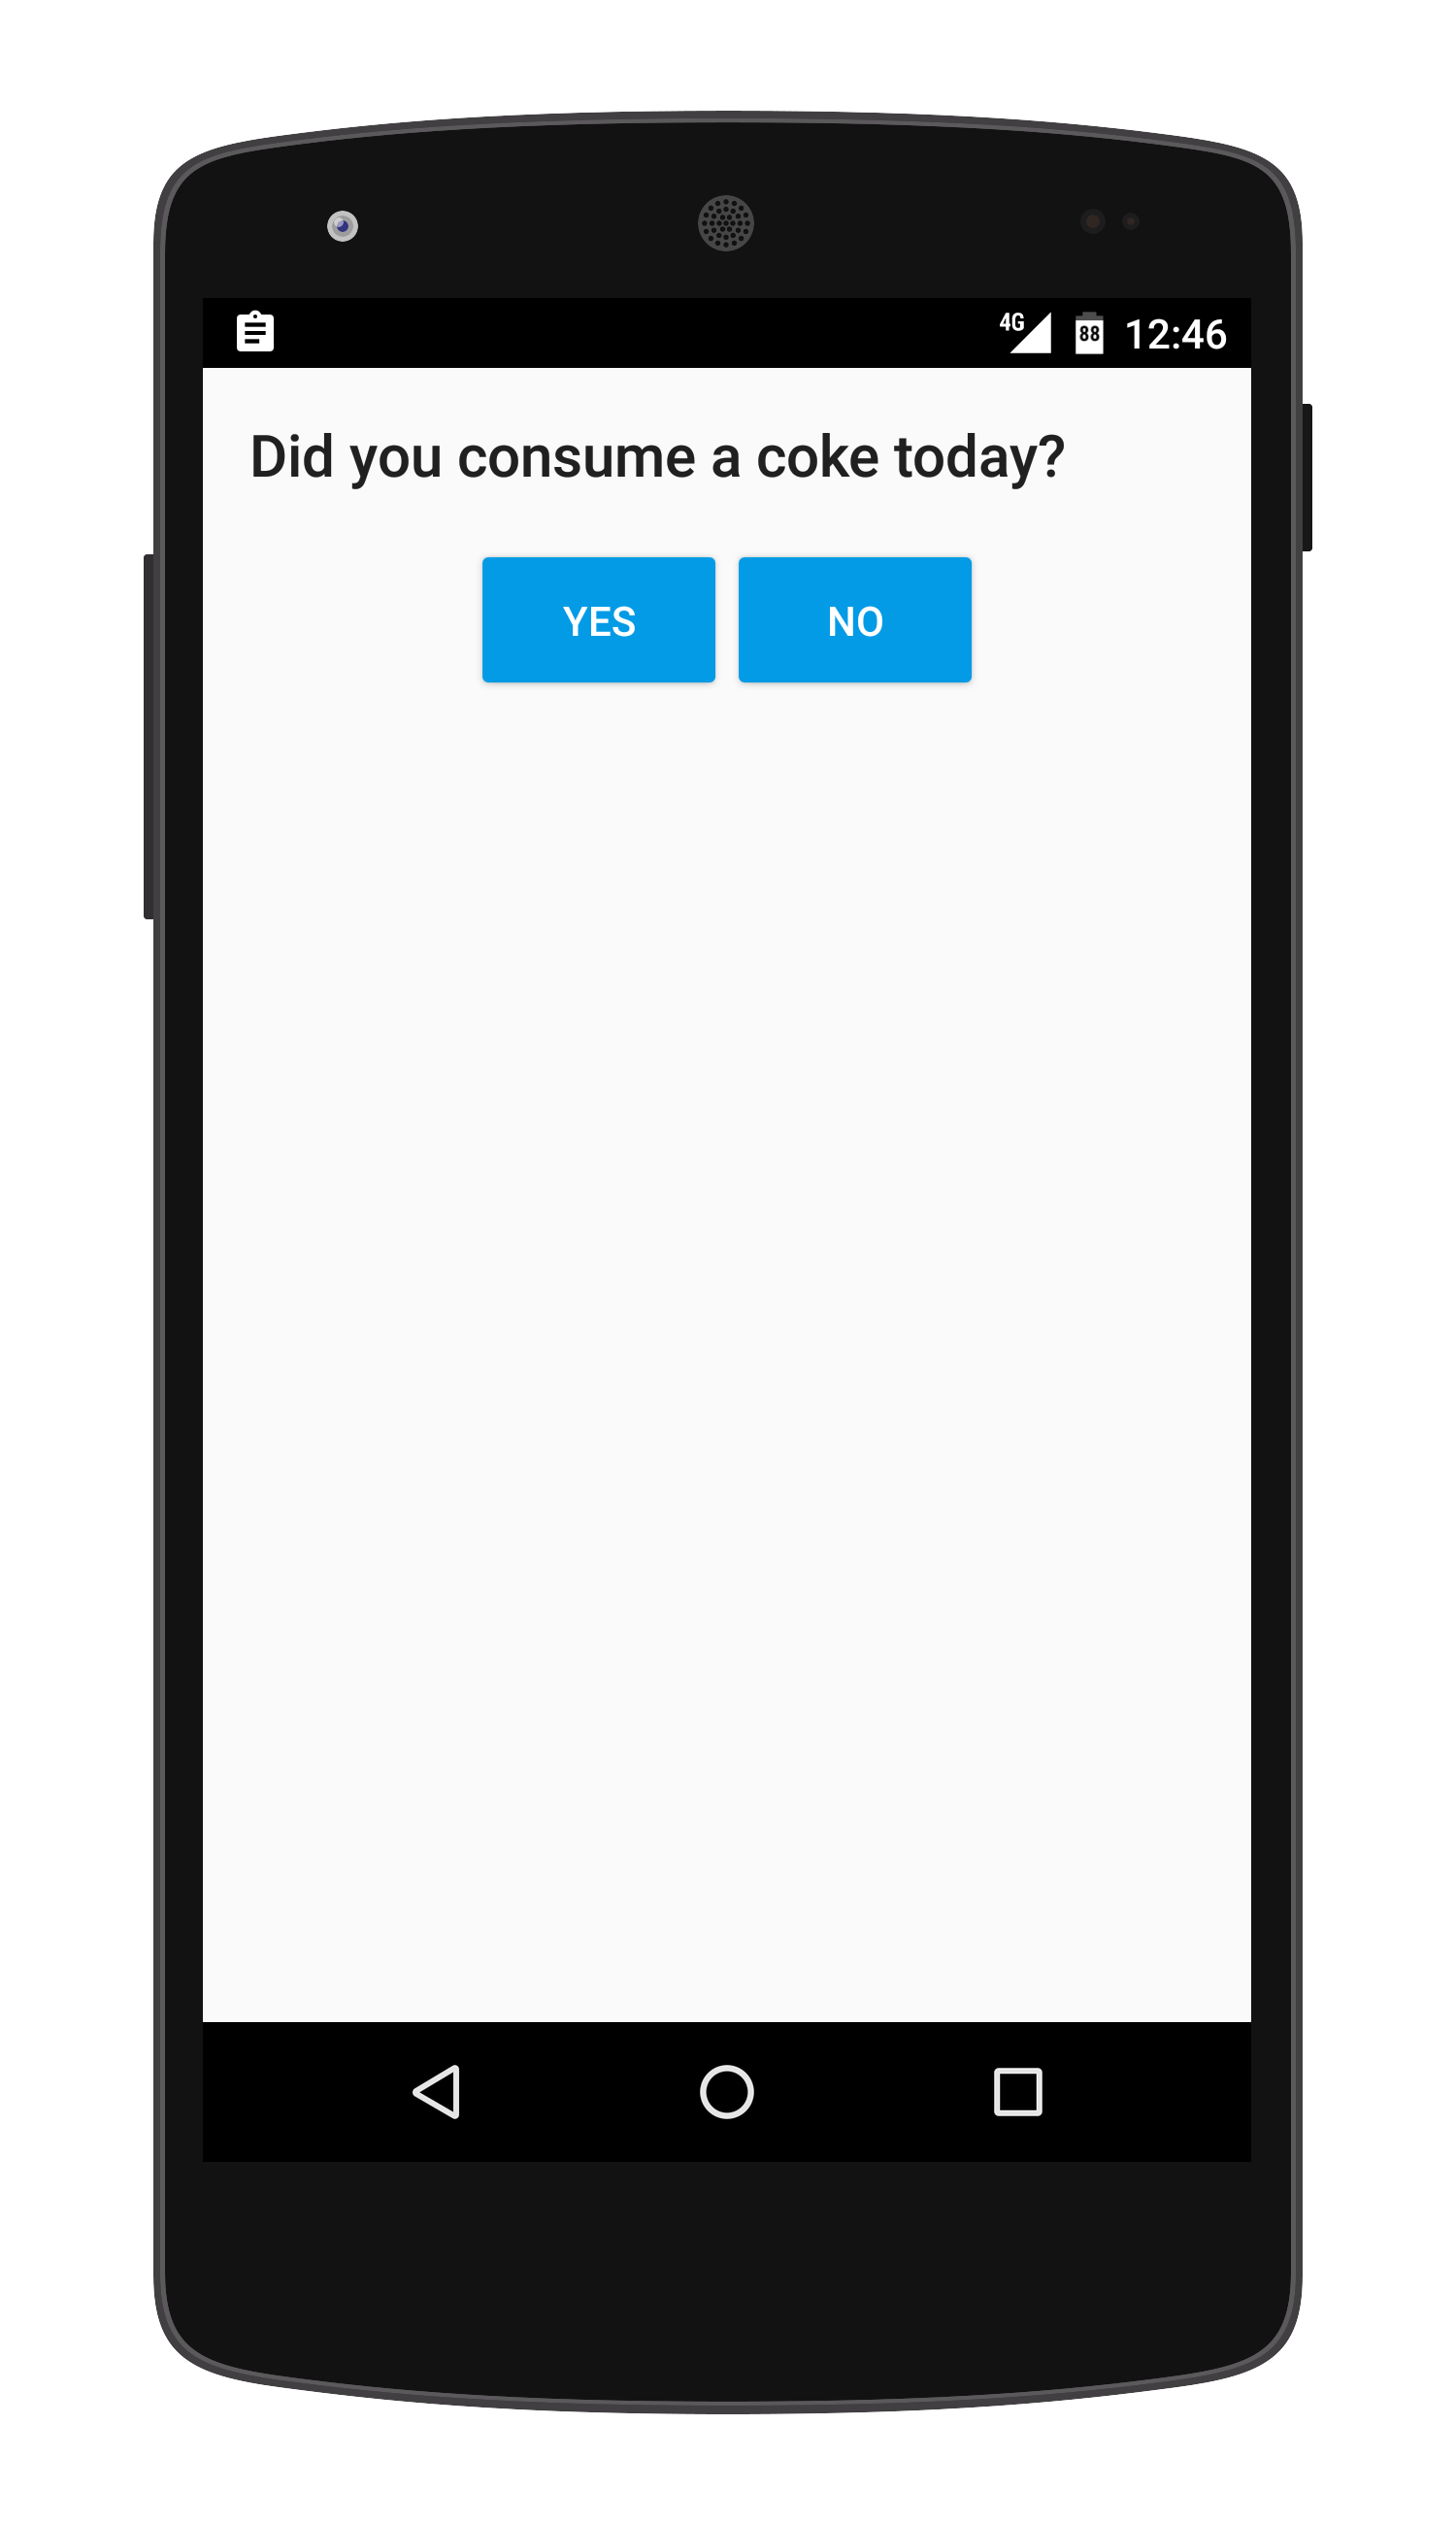
\includegraphics[width=.73\linewidth]{user_interfaces/client/client_answering_questions_with_phone}
        \caption{View when answering a question.}
        \label{fig:answering_questionnaire_answering}
    \end{subfigure}
    \caption{Notification regarding questionnaire is ready to be answered and view of a question being answered.}
    \label{fig:answering_questionnaire}
\end{figure}
\FloatBarrier

In the current system, customers can only specify yes/no questions, but we have thought of different concepts for labeling the collected information.

\begin{description}
    \item[Complex questions] might be required for customers to get a better understanding of the label. Currently, only yes/no questions can be included in a questionnaire, however, customers might be interested to ask more complex questions, such as: \emph{Which of the following statements would describe your current situation best?} or \emph{Please provide a small description of your current mood}. Questions such as the latter might be harder for customers to interpret, but techniques such as  sentiment analysis could be applied here. Ideally, the system should not limit the customer in defining what label they would like to retrieve, i.e. customers should be able to define their own kind of question, or activity, they wish for participants to perform \todo{Her vil jeg gerne beskrive at der er mange metoder som kunderne kan bruge for at få information omkring dataen - så vi skal ikke spænde ben for dem på nogen som helst måde. Måske skal vi evt. overveje om vi skal skrive at de selv kan skrive activities?}. 

    \item[Answer dependent questions] might be desired by customers to get a more detailed label, e.g. if the participants answers \emph{yes} to $q_1$, ask him $q_2$, otherwise ask $q_3$. Defining questions depending on the outcome of previous questions could become a complex task, and the customers might need some aid to visualize the questionnaire. Decision diagrams could be useful for this.
\end{description}

In the current application, questionnaires are triggered, and showed to the user, either in the start or the end of a snapshot \todo{insæt reference}. This will cause the time of questionnaires to be relative to the time that the participants subscribed to the campaign. This might complicate things when trying to build a machine intelligence based model around the collected data, because the label, and time of data collection is skewed between contributers. Because of this, alternative triggers could be desired by customers; some of our considerations are described below.

\begin{description}
    \item[Timely fixed triggers] might be useful to ensure that all participants are notified regarding questionnaires simultaneously, i.e. at a specific time of day. This might cause gathered information to be more easily related. Furthermore, customers might be interested in asking participants regarding something, only at a specific time, e.g. in the morning (after finishing sleeping). 

    \item[Event triggers] could be useful since participants is answering questions based on their own memory. So instead of waiting a fixed amount of time, triggers could be event based. This would prompt participants to answer questionnaires when a specific even occurs, e.g. when returning home, finished a call, etc.    
\end{description}    
